\documentclass[mstat,12pt]{unswthesis}
\usepackage{array}
\usepackage{color}
\usepackage{fancyvrb}
\usepackage{longtable}
\usepackage{tabularx}
\usepackage{caption}
\usepackage{geometry}
\usepackage{booktabs}
\newcommand{\VerbBar}{|}
\newcommand{\VERB}{\Verb[commandchars=\\\{\}]}
\DefineVerbatimEnvironment{Highlighting}{Verbatim}{commandchars=\\\{\}}
% Add ',fontsize=\small' for more characters per line
\usepackage{framed}
\definecolor{shadecolor}{RGB}{248,248,248}
\newenvironment{Shaded}{\begin{snugshade}}{\end{snugshade}}
\newcommand{\AlertTok}[1]{\textcolor[rgb]{0.94,0.16,0.16}{#1}}
\newcommand{\AnnotationTok}[1]{\textcolor[rgb]{0.56,0.35,0.01}{\textbf{\textit{#1}}}}
\newcommand{\AttributeTok}[1]{\textcolor[rgb]{0.77,0.63,0.00}{#1}}
\newcommand{\BaseNTok}[1]{\textcolor[rgb]{0.00,0.00,0.81}{#1}}
\newcommand{\BuiltInTok}[1]{#1}
\newcommand{\CharTok}[1]{\textcolor[rgb]{0.31,0.60,0.02}{#1}}
\newcommand{\CommentTok}[1]{\textcolor[rgb]{0.56,0.35,0.01}{\textit{#1}}}
\newcommand{\CommentVarTok}[1]{\textcolor[rgb]{0.56,0.35,0.01}{\textbf{\textit{#1}}}}
\newcommand{\ConstantTok}[1]{\textcolor[rgb]{0.00,0.00,0.00}{#1}}
\newcommand{\ControlFlowTok}[1]{\textcolor[rgb]{0.13,0.29,0.53}{\textbf{#1}}}
\newcommand{\DataTypeTok}[1]{\textcolor[rgb]{0.13,0.29,0.53}{#1}}
\newcommand{\DecValTok}[1]{\textcolor[rgb]{0.00,0.00,0.81}{#1}}
\newcommand{\DocumentationTok}[1]{\textcolor[rgb]{0.56,0.35,0.01}{\textbf{\textit{#1}}}}
\newcommand{\ErrorTok}[1]{\textcolor[rgb]{0.64,0.00,0.00}{\textbf{#1}}}
\newcommand{\ExtensionTok}[1]{#1}
\newcommand{\FloatTok}[1]{\textcolor[rgb]{0.00,0.00,0.81}{#1}}
\newcommand{\FunctionTok}[1]{\textcolor[rgb]{0.00,0.00,0.00}{#1}}
\newcommand{\ImportTok}[1]{#1}
\newcommand{\InformationTok}[1]{\textcolor[rgb]{0.56,0.35,0.01}{\textbf{\textit{#1}}}}
\newcommand{\KeywordTok}[1]{\textcolor[rgb]{0.13,0.29,0.53}{\textbf{#1}}}
\newcommand{\NormalTok}[1]{#1}
\newcommand{\OperatorTok}[1]{\textcolor[rgb]{0.81,0.36,0.00}{\textbf{#1}}}
\newcommand{\OtherTok}[1]{\textcolor[rgb]{0.56,0.35,0.01}{#1}}
\newcommand{\PreprocessorTok}[1]{\textcolor[rgb]{0.56,0.35,0.01}{\textit{#1}}}
\newcommand{\RegionMarkerTok}[1]{#1}
\newcommand{\SpecialCharTok}[1]{\textcolor[rgb]{0.00,0.00,0.00}{#1}}
\newcommand{\SpecialStringTok}[1]{\textcolor[rgb]{0.31,0.60,0.02}{#1}}
\newcommand{\StringTok}[1]{\textcolor[rgb]{0.31,0.60,0.02}{#1}}
\newcommand{\VariableTok}[1]{\textcolor[rgb]{0.00,0.00,0.00}{#1}}
\newcommand{\VerbatimStringTok}[1]{\textcolor[rgb]{0.31,0.60,0.02}{#1}}
\newcommand{\WarningTok}[1]{\textcolor[rgb]{0.56,0.35,0.01}{\textbf{\textit{#1}}}}
\newcolumntype{Y}{>{\raggedright\arraybackslash}X}


%%%%%%%%%%%%%%%%%%%%%%%%%%%%%%%%%%%%%%%%%%%%%%%%%%%%%%%%%%%%%%%%%%
% 
% OK...Now we get to some actual input.  The first part sets up
% the title etc that will appear on the front page
%
%%%%%%%%%%%%%%%%%%%%%%%%%%%%%%%%%%%%%%%%%%%%%%%%%%%%%%%%%%%%%%%%%

\title{Projet TER par l'équipe 2\\[0.5cm]Rapport de TER, Projet Artist Run Spaces}

\authornameonly{Adjimon Vitoffodji, Anas Jebali, Aya Karami, Noah Guyon, Mohamed Amine El Oualydy}

\author{\Authornameonly}

\copyrightfalse
\figurespagefalse
\tablespagefalse

%%%%%%%%%%%%%%%%%%%%%%%%%%%%%%%%%%%%%%%%%%%%%%%%%%%%%%%%%%%%%%%%%
%
%  And now the document begins
%  The \beforepreface and \afterpreface commands puts the
%  contents page etc in
%
%%%%%%%%%%%%%%%%%%%%%%%%%%%%%%%%%%%%%%%%%%%%%%%%%%%%%%%%%%%%%%%%%%


%%%%%%%%%%%%%%%%%%%%%%%%%%%%%%%%%%%%%%%%%%%%%%%%%%%%%%%%%%%%%%%%%%%%%%%
%
%  A small sample UNSW Coursework Masters thesis file.
%  Any questions to Ian Doust i.doust@unsw.edu.au and/or Gery Geenens ggeenens@unsw.edu.au
%
%%%%%%%%%%%%%%%%%%%%%%%%%%%%%%%%%%%%%%%%%%%%%%%%%%%%%%%%%%%%%%%%%%%%%%%
%
%  The first part pulls in a UNSW Thesis class file.  This one is
%  slightly nonstandard and has been set up to do a couple of
%  things automatically
%
 
%%%%%%%%%%%%%%%%%
%% Precisely one of the next four lines should be uncommented.
%% Choose the one which matches your degree, uncomment it, and comment out the other two!
%\documentclass[mfin,12pt]{unswthesis}    %%  For Master of Financial Mathematics 
%\documentclass[mmath,12pt]{unswthesis}   %%  For Master of Mathematics
%\documentclass[mstat,12pt]{unswthesis}  %%  For Master of Statistics
%%%%%%%%%%%%%%%%%



\linespread{1}
\usepackage{amsfonts}
\usepackage{amssymb}
\usepackage{amsthm}
\usepackage{latexsym,amsmath}
\usepackage{graphicx}
\usepackage{afterpage}
\usepackage[colorlinks]{hyperref}
 \hypersetup{
     colorlinks=true,
     linkcolor=blue,
     filecolor=blue,
     citecolor= black,      
     urlcolor=cyan,
     }
\usepackage{textcomp}
\usepackage{longtable}
\usepackage{booktabs}
\usepackage{float}
\let\origfigure\figure
\let\endorigfigure\endfigure
\renewenvironment{figure}[1][2] {
    \expandafter\origfigure\expandafter[H]
} {
    \endorigfigure
}
\usepackage[T1]{fontenc}
\usepackage{ragged2e}
\def\tightlist{}

%%%%%%%%%%%%%%%%%%%%%%%%%%%%%%%%%%%%%%%%%%%%%%%%%%%%%%%%%%%%%%%%%
%
%  The following are some simple LaTeX macros to give some
%  commonly used letters in funny fonts. You may need more or less of
%  these
%
\newcommand{\R}{\mathbb{R}}
\newcommand{\Q}{\mathbb{Q}}
\newcommand{\C}{\mathbb{C}}
\newcommand{\N}{\mathbb{N}}
\newcommand{\F}{\mathbb{F}}
\newcommand{\PP}{\mathbb{P}}
\newcommand{\T}{\mathbb{T}}
\newcommand{\Z}{\mathbb{Z}}
\newcommand{\B}{\mathfrak{B}}
\newcommand{\BB}{\mathcal{B}}
\newcommand{\M}{\mathfrak{M}}
\newcommand{\X}{\mathfrak{X}}
\newcommand{\Y}{\mathfrak{Y}}
\newcommand{\CC}{\mathcal{C}}
\newcommand{\E}{\mathbb{E}}
\newcommand{\cP}{\mathcal{P}}
\newcommand{\cS}{\mathcal{S}}
\newcommand{\A}{\mathcal{A}}
\newcommand{\ZZ}{\mathcal{Z}}
%%%%%%%%%%%%%%%%%%%%%%%%%%%%%%%%%%%%%%%%%%%%%%%%%%%%%%%%%%%%%%%%%%%%%
%
% The following are much more esoteric commands that I have left in
% so that this file still processes. Use or delete as you see fit
%
\newcommand{\bv}[1]{\mbox{BV($#1$)}}
\newcommand{\comb}[2]{\left(\!\!\!\begin{array}{c}#1\\#2\end{array}\!\!\!\right)
}
\newcommand{\Lat}{{\rm Lat}}
\newcommand{\var}{\mathop{\rm var}}
\newcommand{\Pt}{{\mathcal P}}
\def\tr(#1){{\rm trace}(#1)}
\def\Exp(#1){{\mathbb E}(#1)}
\def\Exps(#1){{\mathbb E}\sparen(#1)}
\newcommand{\floor}[1]{\left\lfloor #1 \right\rfloor}
\newcommand{\ceil}[1]{\left\lceil #1 \right\rceil}
\newcommand{\hatt}[1]{\widehat #1}
\newcommand{\modeq}[3]{#1 \equiv #2 \,(\text{mod}\, #3)}
\newcommand{\rmod}{\,\mathrm{mod}\,}
\newcommand{\p}{\hphantom{+}}
\newcommand{\vect}[1]{\mbox{\boldmath $ #1 $}}
\newcommand{\reff}[2]{\ref{#1}.\ref{#2}}
\newcommand{\psum}[2]{\sum_{#1}^{#2}\!\!\!'\,\,}
\newcommand{\bin}[2]{\left( \begin{array}{@{}c@{}}
				#1 \\ #2
			\end{array}\right)	}
%
%  Macros - some of these are in plain TeX (gasp!)
%
\newcommand{\be}{($\beta$)}
\newcommand{\eqp}{\mathrel{{=}_p}}
\newcommand{\ltp}{\mathrel{{\prec}_p}}
\newcommand{\lep}{\mathrel{{\preceq}_p}}
\def\brack#1{\left \{ #1 \right \}}
\def\bul{$\bullet$\ }
\def\cl{{\rm cl}}
\let\del=\partial
\def\enditem{\par\smallskip\noindent}
\def\implies{\Rightarrow}
\def\inpr#1,#2{\t \hbox{\langle #1 , #2 \rangle} \t}
\def\ip<#1,#2>{\langle #1,#2 \rangle}
\def\lp{\ell^p}
\def\maxb#1{\max \brack{#1}}
\def\minb#1{\min \brack{#1}}
\def\mod#1{\left \vert #1 \right \vert}
\def\norm#1{\left \Vert #1 \right \Vert}
\def\paren(#1){\left( #1 \right)}
\def\qed{\hfill \hbox{$\Box$} \smallskip}
\def\sbrack#1{\Bigl \{ #1 \Bigr \} }
\def\ssbrack#1{ \{ #1 \} }
\def\smod#1{\Bigl \vert #1 \Bigr \vert}
\def\smmod#1{\bigl \vert #1 \bigr \vert}
\def\ssmod#1{\vert #1 \vert}
\def\sspmod#1{\vert\, #1 \, \vert}
\def\snorm#1{\Bigl \Vert #1 \Bigr \Vert}
\def\ssnorm#1{\Vert #1 \Vert}
\def\sparen(#1){\Bigl ( #1 \Bigr )}

\newcommand\blankpage{%
    \null
    \thispagestyle{empty}%
    \addtocounter{page}{-1}%
    \newpage}

%%%%%%%%%%%%%%%%%%%%%%%%%%%%%%%
%
% These environments allow you to get nice numbered headings
%  for your Theorems, Definitions etc.  
%
%  Environments
%
%%%%%%%%%%%%%%%%%%%%%%%%%%%%%%%

\newtheorem{theorem}{Theorem}[section]
\newtheorem{lemma}[theorem]{Lemma}
\newtheorem{proposition}[theorem]{Proposition}
\newtheorem{corollary}[theorem]{Corollary}
\newtheorem{conjecture}[theorem]{Conjecture}
\newtheorem{definition}[theorem]{Definition}
\newtheorem{example}[theorem]{Example}
\newtheorem{remark}[theorem]{Remark}
\newtheorem{question}[theorem]{Question}
\newtheorem{notation}[theorem]{Notation}
\numberwithin{equation}{section}

%%%%%%%%%%%%%%%%%%%%%%%%%%%%%%%%%%%%%%%%%%%%%%%%%%%%%%%%%%%%%%%%%%
%
%  If you've got some funny special words that LaTeX might not
% hyphenate properly, you can give it a helping hand:
%

\hyphenation{Mar-cin-kie-wicz Rade-macher}


\newlength{\cslhangindent}
\setlength{\cslhangindent}{1.5em}
\newlength{\csllabelwidth}
\setlength{\csllabelwidth}{3em}
\newenvironment{CSLReferences}[3] % #1 hanging-ident, #2 entry spacing
 {% don't indent paragraphs
  \setlength{\parindent}{0pt}
  % turn on hanging indent if param 1 is 1
  \ifodd #1 \everypar{\setlength{\hangindent}{\cslhangindent}}\ignorespaces\fi
  % set entry spacing
  \ifnum #2 > 0
  \setlength{\parskip}{#2\baselineskip}
  \fi
 }%
 {}
\usepackage{calc} % for \widthof, \maxof
\newcommand{\CSLBlock}[1]{#1\hfill\break}
\newcommand{\CSLLeftMargin}[1]{\parbox[t]{\maxof{\widthof{#1}}{\csllabelwidth}}{#1}}
\newcommand{\CSLRightInline}[1]{\parbox[t]{\linewidth}{#1}}
\newcommand{\CSLIndent}[1]{\hspace{\cslhangindent}#1}






\renewcommand{\contentsname}{Table des matières}

\renewcommand{\chaptername}{Chapitre}
\geometry{left=2.5cm, right=2.5cm, top=2.5cm, bottom=2.5cm}

% Définit un nouveau type de colonne X pour texte justifié avec bordures visibles
\newcolumntype{L}[1]{>{\raggedright\arraybackslash}p{#1}}


\begin{document}

\beforepreface
%\afterpage{\blankpage}

% plagiarism

\prefacesection{Déclaration de non plagiat}

\vskip 2pc \noindent Nous déclarons que ce rapport est le fruit de notre seul travail, à part lorsque cela est indiqué  explicitement. 

\vskip 2pc  \noindent Nous acceptons que la personne évaluant ce rapport puisse, pour les besoins de cette évaluation:
\begin{itemize}
\item la reproduire et en fournir une copie à un autre membre de l'université; et/ou,
\item en communiquer une copie à un service en ligne de détection de plagiat (qui pourra en retenir une copie pour les besoins d'évaluation future).
\end{itemize}

\vskip 2pc \noindent Nous certifions que nous avons lu et compris les règles ci-dessus.\vspace{24pt}

\vskip 2pc \noindent En signant cette déclaration, nous acceptons ce qui précède.
\vskip 2pc \noindent
Signature: Adjimon Vitoffodji \hfill Date: 12/05/2025 \\[1cm]
Signature: Anas Jebali \hfill Date: 12/05/2025 \\[1cm]
Signature: Aya Karami \hfill Date: 12/05/2025 \\[1cm]
Signature: Noah Guyon \hfill Date: 12/05/2025 \\[1cm]
\vskip 1pc
%\afterpage{\blankpage}

% Acknowledgements are optional


\prefacesection{Remerciements}
\vspace{7 cm}
Nous adressons nos plus sincères remerciements à notre encadrant pédagogique dont les conseils judicieux et l'accompagnement attentif ont considérablement enrichi notre démarche tout au long de ce projet.

\vspace{0.5 cm} 

Nous tenons également à exprimer notre profonde gratitude envers François-David Collin et Sabrina Issa, dont l'expertise précieuse, la disponibilité constante et les perspectives éclairantes ont été déterminantes dans l'aboutissement de ce travail. Leur soutien bienveillant et leurs contributions substantielles ont fait de cette expérience un véritable parcours d'apprentissage et de développement intellectuel.

{\bigskip\bigskip\bigskip\noindent} \today

%\afterpage{\blankpage}

% Abstract

\prefacesection{Résumé}

\vspace{2cm}

\begin{center}
\begin{minipage}{0.85\textwidth}
\setlength{\parindent}{0pt}
\setlength{\parskip}{0.5em}

Ce rapport présente une analyse approfondie des \textit{artist-run spaces} — ces espaces artistiques autogérés qui constituent un phénomène culturel significatif mais encore insuffisamment documenté. Notre recherche mobilise les techniques avancées de la data science pour explorer, classifier et cartographier ces lieux selon des dimensions multiples.

L'étude déploie une méthodologie hybride combinant analyse géospatiale, exploration temporelle et traitement du langage naturel. Cette approche nous permet d'identifier des tendances émergentes dans la distribution et l'évolution de ces espaces à l'échelle mondiale.

Notre contribution majeure réside dans la construction d'une base de données multilingue enrichie, conçue spécifiquement pour capturer la complexité et la diversité de ces initiatives artistiques. L'implémentation d'algorithmes comme BERT pour le traitement des données textuelles a significativement amélioré notre capacité à extraire et analyser des informations pertinentes à partir de sources hétérogènes.

Ce travail ouvre des perspectives nouvelles pour la compréhension des écosystèmes artistiques alternatifs et leur intégration dans les politiques culturelles contemporaines.

\end{minipage}
\end{center}

\vspace{2cm}

\par


%\afterpage{\blankpage}


\afterpreface

\listoffigures
\listoftables




%%%%%%%%%%%%%%%%%%%%%%%%%%%%%%%%%%%%%%%%%%%%%%%%%%%%%%%%%%%%%%%%%%
%
% Now we can start on the first chapter
% Within chapters we have sections, subsections and so forth
%
%%%%%%%%%%%%%%%%%%%%%%%%%%%%%%%%%%%%%%%%%%%%%%%%%%%%%%%%%%%%%%%%%%



%%%%%%%%%%%%%%%%%%%%%%%%%%%%%%%%%%%%%

%\afterpage{\blankpage}


\hypertarget{introduction}{%
\chapter{Introduction}\label{introduction}}

\hypertarget{contenu-dune-introduction}{%
\section{Contenu d'une introduction}\label{contenu-dune-introduction}}

Les artist-run spaces sont des lieux autogérés où les artistes organisent et exposent
leurs propres créations, un phénomène unique dans l’art contemporain. Dans le
cadre de notre projet TER, coordonné par des experts comme François-David
Collin et Sabrina Issa, vise à explorer ces lieux au-delà des classifications traditionnelles. Notre équipe a beaucoup discuté des différents aspects de ce projet, qui,
bien que fascinant, présente des défis importants. Nous avons naturellement réparti
les tâches, chaque membre contribuant à l’ensemble des étapes. Les discussions se
font toujours en groupe pour assurer que chacun reste aligné sur les avancées et
objectifs. Cette approche nous permet de combiner nos perspectives et d’adapter
notre progression en fonction des résultats observés. L’étude des artist-run spaces
se concentre sur l’évolution de ces espaces au fil du temps et à travers des zones
géographiques diverses, en tentant de cartographier des tendances souvent invisibles dans les données brutes. Ces lieux se différencient par leur flexibilité et leur
résilience, rendant leur documentation importante pour préserver leur influence et
leur impact social. Le projet utilise des outils permettant d’étudier l’impact de ces
espaces selon des critères tels que l’emplacement, le type d’activité, et les périodes
d’ouverture/fermeture. Notre équipe a adopté une approche pour structurer le projet en trois étapes principales : extraction et nettoyage des données, analyse et
modélisation, et visualisation. Des visualisations rendront les résultats accessibles,
ce qui offre une meilleure compréhension de l’évolution et de l’impact des artist-run
spaces.
Pour ce second semestre, nous avons commencé par retravailler notre compréhension du corpus de descriptions d'espaces, en analysant les mots les plus présents dans les textes. Ensuite nous avons redéveloppé une base plus correcte pour l'utilisation de nos données et enfin nous avons commencé les modèles de topixification pour classer les espaces d'art.




\hypertarget{revue-de-la-littuxe9rature}{%
\chapter{Revue de la littérature}\label{revue-de-la-littuxe9rature}}
\vspace{4 cm}
\hypertarget{contenu-de-luxe9tat-de-lart}{%
\section{Contenu de l'état de l'art}\label{contenu-de-luxe9tat-de-lart}}

Ce projet aborde un sujet à la fois novateur et contemporain, pour lequel il existe peu de communications ou de travaux antérieurs. En effet, les seules personnes ayant travaillé sur cette thématique sont nos encadrants ainsi que leurs collaborateurs dans le cadre du projet Artist-Run Spaces, ainsi que l’équipe MIASHS du Marathon du Web 2019/2020.
\vspace{1 cm}
Les seuls travaux en data science identifiés sont ceux réalisés par cette dernière équipe.
Leur étude portait sur l’analyse des espaces d’art et de leur proximité, comparée à leur description. Leur objectif était relativement proche du nôtre, bien qu’il diffère sur certains points. En effet, notre but est de pouvoir classifier ces espaces en fonction de thématiques spécifiques (et non générales), afin d’obtenir des classes précises, que nous nommons topics.

\hypertarget{matuxe9riel-et-muxe9thodes}{%
\chapter{Matériel et Méthodes}\label{matuxe9riel-et-muxe9thodes}}

\hypertarget{Gestion de projet}{%
\section{Gestion de projet}\label{Gestion de projet}}

Aya, notre Team Leader, a veillé à ce que l’ensemble des membres de l’équipe travaillent de manière synchronisée, en coordonnant les efforts et en répartissant les tâches selon les compétences et affinités de chacun. Cette organisation s’inscrit dans une démarche de gestion de projet en méthode agile, favorisant la flexibilité, l’adaptation continue et le travail collaboratif. La répartition des rôles a été facilitée par l’élaboration d’un graphe collaboratif, mettant en évidence les expertises de chaque membre, notamment en visualisation, en traitement de textes et en développement Python. Nous avons fonctionné par itérations courtes, avec des objectifs définis à chaque réunion et des ajustements réguliers en fonction de l’avancement du projet et des retours de notre tuteur. Aya joue également un rôle dans le suivi et la dynamique de groupe, en identifiant les éventuels blocages et en veillant à maintenir une communication bienveillante au sein de l’équipe. Les réunions sont fixées via Discord, qui sert également d’outil centralisé pour les échanges quotidiens et l’archivage des discussions. L’équipe se réunit au minimum une fois par semaine pour faire le point sur les avancées, en plus d’une réunion hebdomadaire avec notre tuteur. À l’issue de chaque rencontre, la coordinatrice rédige un compte rendu détaillant les actions effectuées, les points abordés et les tâches à réaliser pour la semaine suivante. Ce bilan est relu et validé par l’ensemble des membres avant d’être déposé sur notre dépôt GitHub afin d’en assurer la traçabilité.

\hypertarget{logiciels}{%
\section{Logiciels}\label{logiciels}}

Dans le cadre de ce projet, nous avons principalement travaillé en Python pour le traitement des données, la modélisation et la création de visualisations. Nous avons mobilisé un ensemble de bibliothèques liées au traitement automatique du langage naturel, en particulier à l’architecture BERT. Parmi celles-ci, sentence-transformers et BERTopic ont été largement utilisées pour l’encodage sémantique des textes et la génération automatique de topics. D’autres bibliothèques comme pandas, numpy, matplotlib ou plotly nous ont permis de manipuler les données et de produire des visualisations claires et interactives. Pour le développement, nous avons utilisé principalement Jupyter Notebooks et Visual Studio Code. Le code a été versionné et archivé sur notre dépôt GitHub, enrichi régulièrement comme au premier semestre. Afin d’optimiser les performances et de réduire les temps de calcul, notamment lors de l’exécution des modèles de topic modeling, nous avons utilisé la machine virtuelle mise à disposition par M. Collin (Ubuntu 22.04, processeur Intel Xeon 2.6 GHz, 32 Go de RAM, Python 3.10). Ce choix d’environnement s’appuie à la fois sur notre expérience antérieure avec ces outils et sur leur efficacité reconnue pour les tâches de traitement de texte. Enfin, la coordination de l’équipe s’est appuyée sur des réunions régulières et l’utilisation d’outils de communication comme Discord.

\hypertarget{description-des-donnuxe9es}{%
\section{Description des Données}\label{description-des-donnuxe9es}}

Les données mobilisées dans ce projet proviennent d’une base recensant des artist-run spaces situés en Europe. Chaque entrée contient des informations textuelles (description, objectifs, activités, etc.), des métadonnées (nom, site web, pays, ville), ainsi que des coordonnées de localisation.
Ces données ont été stockées sous forme de fichiers JSON et CSV, organisés dans des dossiers thématiques selon la source ou la nature du contenu (base principale, textes complémentaires, entrées modifiées, etc.).

\hypertarget{nettoyage-des-donnuxe9es}{%
\section{Nettoyage des données}\label{nettoyage-des-donnuxe9es}}

Extraction des informations : Les données textuelles et de localisation ont été extraites à partir de la base existante.

Nettoyage : Une première phase de nettoyage a permis d’uniformiser les formats, corriger les incohérences (valeurs manquantes, balises HTML, doublons), et enrichir certaines entrées avec des métadonnées supplémentaires.

Transformation pour visualisation : Les données ont été restructurées avec des frameworks Python (tels que pandas et json) en vue de leur intégration dans des outils de visualisation comme D3.js.

Vers la fin du second semestre, un incident technique sur le serveur a entraîné la suppression involontaire d’une partie des données. Après récupération, ces fichiers ont fait l’objet d’un nouveau nettoyage rigoureux : suppression des balises HTML résiduelles, traitement des valeurs nulles, uniformisation des formats. Nous avons également utilisé la bibliothèque SpaCy pour certaines opérations de normalisation linguistique, telles que la lemmatisation et la suppression des stopwords. Enfin, afin d’unifier l’ensemble du corpus et de le rendre compatible avec les modèles linguistiques préentraînés, les données ont été traduites en anglais.

\hypertarget{uxe9tapes-de-pruxe9-traitements}{%
\section{Étapes de
Pré-traitements}\label{uxe9tapes-de-pruxe9-traitements}}

Les données ont subi plusieurs transformations afin de les rendre exploitables pour les analyses textuelles et visuelles. Parmi ces étapes figurent :

Nettoyage linguistique : suppression des balises HTML, ponctuations superflues, valeurs nulles ou redondantes.

Normalisation textuelle : conversion en minuscules, lemmatisation, suppression des stopwords, parfois à l’aide de SpaCy.

Traduction automatique : les textes ont été traduits en anglais pour garantir la compatibilité avec les modèles NLP tels que BERTopic ou sentence-transformers, principalement entraînés sur des corpus anglophones.

Structuration des données : reformattage en dictionnaires ou DataFrames, en vue de leur exploitation dans les modèles d’analyse ou les visualisations interactives.


\hypertarget{muxe9thodologie-de-luxe9valuation}{%
\section{Méthodologie de l'évaluation}\label{muxe9thodologie-de-luxe9valuation}}

Pour répondre aux objectifs du projet, la méthodologie s'appuie sur des techniques de traitement automatique du langage naturel (TALN), de clustering, d'analyse de réseaux, et de visualisation interactive, appliquées à l'analyse de corpus textuels spécialisés.

\subsection{préparation des données}

La première étape a consisté à charger les données à partir du fichier Excel new-fichier-traduit.xlsx, contenant des informations sur les espaces culturels, telles que leur nom, leurs coordonnées géographiques (latitude et longitude), leur ville, leur pays, leur site web, ainsi que des textes descriptifs (activités, présentation, historique, réponses à des questions). Le fichier a été lu à l'aide de la bibliothèque pandas avec le moteur openpyxl.
Pour évaluer la complétion des données, un diagramme circulaire a été généré afin de visualiser le taux de réponses. Les espaces ayant répondu à au moins une question ont été distingués de ceux sans réponse, et ces statistiques ont été sauvegardées dans un fichier JSON (reponses\_stats.json) pour une utilisation ultérieure dans l'interface React.

\subsection{Prétraitement des textes}

Les textes des différentes colonnes (activites, presentation, historique, réponse1, réponse2) ont été combinés pour chaque espace en une seule colonne texte-combine à l'aide d'une fonction personnalisée combine-columns.
Ensuite, une fonction de prétraitement plus approfondie, pour Convertir les textes en minuscules, Supprimer les URLs et les caractères spéciaux (par exemple, via des expressions régulières), Exclure les nombres courts (sauf les années), Retirer les mots vides (stopwords) en anglais et français, ainsi qu'une liste personnalisée de mots non pertinents (custom\_stop\_words), Normaliser certains noms propres (par exemple, en remplaçant les noms d'organisations par un placeholder générique ART-ORG).
Un DataFrame final processed\_df a été créé, contenant uniquement les espaces avec un texte combiné non vide et d'une longueur minimale de 20 mots, afin de garantir une analyse textuelle pertinente. Ce DataFrame a été sauvegardé dans processed\_df\_backup.csv pour référence.

\subsection{Génération d'un nuage de mots}

Pour identifier les termes les plus fréquents dans les textes des espaces, un nuage de mots a été généré à l'aide de la bibliothèque WordCloud. Les textes de tous les espaces ont été concaténés en un seul corpus, et les mots vides anglais (via nltk.corpus.stopwords) ainsi qu'une liste de mots personnalisés non pertinents (par exemple, "also", "would") ont été exclus. Le nuage de mots a été configuré pour inclure jusqu'à 100 mots, avec des paramètres visuels tels qu'une largeur de 800 pixels, une hauteur de 400 pixels, un fond blanc, et une colormap viridis. Les mots et leurs fréquences normalisées ont été extraits et sauvegardés dans un fichier JSON (word\_cloud\_data.json) pour une visualisation interactive dans React.
Une image statique (word\_cloud.png) a également été générée pour référence.

\subsection{Modélisation des Topics BERTopic}

L'identification des thématiques a été réalisée à l'aide de la bibliothèque BERTopic, qui combine des embeddings de texte, une réduction de dimensionnalité, un clustering, et une 
extraction de mots-clés.

\bigskip

\subsubsection{3.6.4.1   Architecture et Paramétrage}

\bigskip

\begin{scriptsize}
\begin{longtable}{@{}p{3.7cm} p{3.9cm} p{5.5cm} p{3.8cm}@{}}
\caption{Architecture du modèle implémenté.\label{tab:modele}} \\
\toprule
\textbf{Composant} & \textbf{Rôle} & \textbf{Paramètres clés} & \textbf{Bibliothèque/Module} \\
\midrule
\endfirsthead

\toprule
\textbf{Composant} & \textbf{Rôle} & \textbf{Paramètres clés} & \textbf{Bibliothèque/Module} \\
\midrule
\endhead

\midrule
\endfoot

\bottomrule
\endlastfoot

Génération des embeddings & Conversion de textes en représentations vectorielles sémantiques. & 
Modèle : \texttt{paraphrase\-multilingual\-MiniLM\-L12\-v2} \newline
Mise en cache des embeddings (\texttt{embeddings\_cache.pkl}) &
\texttt{SentenceTransformer} \\

Réduction de dimensionnalité (UMAP) & Réduction des dimensions des embeddings pour faciliter le clustering. &
\texttt{n\_neighbors=5} \newline
\texttt{n\_components=5} \newline
\texttt{min\_dist=0.0} \newline
\texttt{metric="cosine"} \newline
\texttt{random\_state=42} & 
\texttt{umap-learn (via UMAP)} \\

Clustering (HDBSCAN) & Regroupement des documents en clusters (topics) basés sur les embeddings. &
\texttt{min\_cluster\_size=2} \newline
\texttt{min\_samples=1} \newline
\texttt{metric="euclidean"} \newline
\texttt{cluster\_selection\_method="eom"} & 
\texttt{hdbscan (via HDBSCAN)} \\

Vectorisation des mots-clés & Extraction et vectorisation des mots-clés pour chaque document. &
\texttt{ngram\_range=(1,3)} \newline
\texttt{stop\_words=custom\_stop\_words} &
\texttt{scikit-learn (via CountVectorizer)} \\

Modèle de représentation (KeyBERTInspired) & Extraction de mots-clés pertinents pour chaque topic. &
\texttt{top\_n\_words=15} &
\texttt{bertopic.representation (via KeyBERTInspired)} \\

Diversification des mots-clés (MMR) & Réduction de la redondance des mots-clés pour une meilleure diversité. &
\texttt{diversity=0.5} &
\texttt{bertopic.representation (via MaximalMarginalRelevance)} \\

Modèle BERTopic & Orchestration du pipeline (embedding, réduction, clustering, représentation des topics). &
\texttt{min\_topic\_size=2} \newline
\texttt{top\_n\_words=10} \newline
\texttt{calculate\_probabilities=True} \newline
\texttt{nr\_topics="auto"} &
\texttt{bertopic (via BERTopic)} \\

Résumés des topics (Mistral Small 3.1) & Génération de résumés concis pour chaque topic. &
Modèle : \texttt{mistral-small-3.1} \newline
\texttt{max\_tokens=150} \newline
\texttt{temperature=0.3} \newline
\texttt{prompt: "Summarize the main theme in one concise sentence (max 15 words)"} &
\texttt{openai (via AsyncOpenAI)} \\

\end{longtable}
\end{scriptsize}


\bigskip

\subsubsection{3.6.4.2   Analyse du choix de l’architecture : }

\bigskip

\begin{enumerate}
    \item Choix du Modèle d'Embeddings
    
    \bigskip

    Le choix du modèle paraphrase-multilingual-MiniLM-L12-v2 résulte d'une analyse
    approfondie des contraintes spécifiques de notre corpus. Premièrement, la dimension 384
    représente un compromis optimal entre expressivité sémantique et efficacité
    computationnelle : elle est suffisamment riche pour capturer les nuances des descriptions
    d'espaces artistiques tout en restant tractable pour l'analyse de 330 documents.
    Deuxièmement, le caractère multilingue s'avère indispensable car notre corpus mélange
    français et anglais de manière imprévisible, et toute étape de traduction préalable
    introduirait inévitablement du bruit et des biais. Enfin, la spécialisation sur les paraphrases
    est particulièrement pertinente dans notre contexte où différents espaces peuvent décrire
    des concepts similaires avec des formulations variées - par exemple, "espace d'art
    contemporain" et "galerie expérimentale" doivent être reconnues comme sémantiquement
    proches.

    \bigskip

    \item Pipeline de Réduction Dimensionnelle :
    
    \bigskip

    L'utilisation d'UMAP avec ces paramètres spécifiques répond à des impératifs techniques et
    théoriques précis. Le paramètre n-neighbors=8 a été soigneusement calibré pour notre taille
    d'échantillon : avec 330 documents, une valeur trop faible (comme 3-5) créerait une surfragmentation en ignorant la structure globale, tandis qu'une valeur trop élevée (>15)
    lisserait excessivement les variations locales importantes pour distinguer les micro-niches
    artistiques. La réduction drastique à 5 composantes (384→5) s'impose pour éviter la
    malédiction dimensionnelle qui affecterait l'efficacité d'HDBSCAN, tout en conservant
    suffisamment d'information pour préserver les relations sémantiques essentielles.
    L'adoption de la métrique cosinus s'explique par sa nature : elle mesure l'angle entre
    vecteurs, capturant ainsi l'orientation sémantique indépendamment de la magnitude, ce qui
    est crucial quand on compare des textes de longueurs très différentes.

    \bigskip


    \item Algorithme de Clustering HDBSCAN

    \bigskip

    Le paramétrage agressif d'HDBSCAN reflète notre objectif d'identifier des niches
    thématiques fines dans le paysage artistique. Le min-cluster-size=2 peut sembler risqué,
    mais il se justifie par la nature exploratoire de notre recherche : nous préférons identifier
    des micro-tendances potentiellement significatives quitte à devoir les valider manuellement,
    plutôt que de les manquer avec un seuil plus conservateur. Le min-samples=1 amplifie cette
    sensibilité**, permettant de détecter des outliers informatifs qui pourraient révéler des
    approches artistiques émergentes ou atypiques. L'utilisation de la méthode EOM (Excess of
    Mass) garantit une sélection robuste en privilégiant les clusters avec la densité la plus
    élevée, ce qui est particulièrement approprié quand on cherche à identifier des
    regroupements conceptuels naturels.

    \bigskip

    \item Stratégie Hybride de Représentation des Topics

    \bigskip

    \begin{enumerate}
        \item KeyBERTInspired : Extraction Contextuelle

        \bigskip

        L'adoption de KeyBERTInspired marque une rupture méthodologique avec les approches traditionnelles comme TF-IDF. Contrairement aux méthodes statistiques classiques, KeyBERTInspired préserve le contexte sémantique BERT tout au long du processus d'extraction, garantissant que les mots-clés sélectionnés reflètent véritablement la sémantique sous-jacente plutôt que de simples fréquences statistiques. Le couplage avec MMR (Maximal Marginal Relevance) avec diversity=0.5 introduit un contrôle fin de la diversité : cette valeur médiane assure un équilibre entre pertinence (similarité au topic) et diversité (évitement de la redondance), particulièrement crucial quand on analyse des discours artistiques où la synonymie et la variabilité expressionnelle sont fréquentes. La génération de scores de confiance pour chaque terme permet une évaluation quantitative de la qualité des mots-clés extraits, facilitant ainsi le post-traitement et la validation.

        \bigskip

        \item Différence entre KeyBERT et KeyBERTInspired :

        \bigskip

        KeyBERT est un outil basé sur des modèles BERT (ou similaires) pour extraire les mots-clés les plus représentatifs d’un texte. Tant disque KeyBERTInspired n’est pas une librairie officielle, mais une implémentation personnalisée ou allégée de KeyBERT, souvent utilisée dans des frameworks ou des bibliothèques comme BERTopic, OctoML, ou des projets internes qui reprennent l'idée de KeyBERT sans utiliser le package original. mais elles diffèrent dans leur conception, leur objectif, et leur intégration dans des pipelines comme BERTopic.


        \begin{table}[H]
        \centering
            \caption{Différence entre KeyBERT et KeyBERTInspired}
            \begin{tabular}{|p{3cm}|p{5cm}|p{5cm}|}
                \hline
                \textbf{Aspect} & \textbf{KeyBERT (original)} & \textbf{KeyBERTInspired} \\
                \hline
                Objet principal & Méthode automomé pour extraire des mots-clés à partir de textes en utilisant des embeddings BERT & Variante optimisée pour BERTopic, conçue pour représenter des topics en extrayant des mots-clés représentatifs \\
                \hline
                Méthodologie & - Utilise des embeddings BERT pour le texte et les mots candidats. - Calcule la similarité cosinus entre les embeddings du document et ceux des mots candidats (généralement des n-grams extraits). - Sélectionne les mots ayant la plus haute similarité comme mots-clés. & - S'inspire de KeyBERT mais est adapté pour BERTopic. - Explore les embeddings des documents d'un topic (après clustering) pour extraire des mots-clés qui représentent les topics. - Utilise une approche plus rapide, optimisée pour les pipelines de topic modeling. \\
                \hline
                Itération & - Plus lent, car il calcule les embeddings pour chaque mot candidat séparément. - Peut être plus précis pour des cas spécifiques nécessitant une extraction fine. & - Plus rapide, car il optimise l'ordre d'exécution dans les pipelines BERTopic. - Maintien précis pour des tâches d'extraction automone, mais s'adapte pour décrire des topics. \\
                \hline
                Personnalisation & Très personnalisable (stop words, modèle, diversité, etc.) & Maintien des paramètres accessibles directement dans BERTopic avec des mécanismes d'optimisation. \\
                \hline
                Diversité des mots-clés & - Peut générer des mots-clés redondants. - Nécessite souvent une post-étape comme Maximal Marginal Relevance (MMR) pour diversifier les résultats. & - Intègre implicitement des mécanismes pour réduire la redondance (surround si combiné avec MMR dans BERTopic). \\
                \hline
                Exemple d'intégration & Utilisé directement dans des projets de NLP & Utilisé comme module de scoring dans BERTopic, par ex. \\
                \hline
            \end{tabular}
            \label{tab:keybert_vs_keybertinspired}
        
        \end{table}

        En conclusion, KeyBERT est une librairie indépendante, polyvalente, et bien documenté,
        tant disque KeyBERTInspired, utilisé comme méthode d’extraction de mots-clés pour les
        topics.

        \bigskip

        \item MMR (Maximal Marginal Relevance)

        \bigskip

        MMR est une méthode de sélection qui équilibre deux choses :
        - La pertinence d’un mot-clé (sa similarité avec le document)
        - La diversité entre les mots-clés (éviter les redondances)
        La formule MMR est généralement :
        \[
        \text{MMR} = \arg\max_{k_i \in R \setminus S} \left[
        \lambda \cdot \text{Sim}(k_i, D) - (1 - \lambda) \cdot \max_{k_j \in S} \text{Sim}(k_i, k_j)
        \right]
        \]
        \begin{align*}
        R &: \text{ ensemble de candidats} \\
        S &: \text{ mots-clés déjà sélectionnés} \\
        D &: \text{ document (ou représentation du document)} \\
        \lambda &\in [0, 1] : \text{ coefficient d’équilibre entre pertinence et diversité}
        \end{align*}
        Donc KeyBERTInspired + MMR, c’est :
        Générer des candidats mots-clés à partir du texte, Utiliser des embeddings (genre BERT)
        pour calculer la similarité et Appliquer MMR pour sélectionner les meilleurs mots-clés
        diversifiés et pertinents.
        
    \end{enumerate}

    \bigskip

    \item Génération de Résumés par LLM

    \bigskip

    L'intégration de Mistral Small 3.1 représente une innovation méthodologique visant à humaniser l'interprétation des topics. Le choix de Mistral Small 3.1 plutôt que des modèles plus volumineux s'explique par son optimisation spécifique pour les tâches de synthèse, offrant un rapport qualité/vitesse optimal pour notre usage. La température de 0.3 a été finement ajustée après plusieurs itérations : plus basse, elle produisait des résumés trop mécaniques ; plus haute, elle introduisait des variations créatives inadaptées à un contexte scientifique. La limitation stricte à 15 tokens force la concision, évitant les descriptions verbeuses tout en exigeant de capturer l'essence du topic - une contrainte qui s'avère souvent révélatrice de la cohérence réelle du cluster. Le système de retry avec backoff exponentiel gère de manière robuste les éventuelles instabilités de l'API locale, garantissant la complétude des résultats même en cas de surcharge temporaire.
\end{enumerate}

\bigskip

\subsection{Évaluation de la qualité des topics}


La qualité des topics a été évaluée à l'aide de deux métriques mathématiques :
\begin{itemize}
 \item \textbf{Diversité des topics} : Cette métrique mesure la proportion de mots-clés
uniques par rapport au total des mots-clés extraits. Elle est définie par la formule suivante :
 \[
 \text{Diversité des topics} = \frac{|\text{U}|}{N}
 \]
 où \( |\text{U}| \) représente le nombre de mots-clés uniques, et \( N \) le nombre total
de mots-clés extraits.
\item Une valeur proche de 1 indique une faible redondance (diversité élevée), tandis
qu'une valeur proche de 0 indique une forte redondance.
 \item \textbf{Couverture des topics} : Cette métrique évalue la proportion de documents
non assignés (topic -1) par rapport au total des documents. Elle est donnée par :
 \[
 \text{Couverture des topics} = \frac{T - C}{T}
 \]
 où \( T \) est le nombre total de documents, et \( C \) le nombre de documents assignés à
des topics valides.
\item Une valeur proche de 0 indique une couverture élevée (peu d'outliers), tandis qu'une
valeur plus élevée indique que le modèle a du mal à assigner des documents à des topics.
\end{itemize}

\subsection{Analyse des relations entre topics}

Les relations entre les topics identifiés à partir des données textuelles des espaces culturels ont été analysées et visualisées de manière approfondie afin de comprendre leur structure sémantique, leur distribution, et leurs interconnexions. Cette analyse a été réalisée à l’aide de plusieurs approches visuelles interactives, chacune offrant une perspective complémentaire sur les relations entre les topics. Les outils principaux utilisés incluent BERTopic pour les visualisations spécifiques aux topics et Plotly pour des représentations interactives personnalisées. Les détails de chaque méthode sont décrits ci-dessous.

\bigskip

\subsubsection{3.6.6.1   Distribution des topics :}

\bigskip
\begin{itemize}
    \item 
    Un diagramme en barres interactif a été généré pour illustrer la distribution des topics en termes de pourcentage de documents associés à chaque topic.
    \item 
    Cette visualisation permet d’identifier les topics dominants (ceux avec le plus grand pourcentage de documents) et de détecter d’éventuelles imbalances dans la répartition des données.
\end{itemize}

\bigskip

\subsubsection{3.6.6.2   Carte des distances entre topics : }

\bigskip

Une visualisation interactive de la distance entre topics a été générée avec la méthode BERTopic.visualize\_topics(), offrant une représentation courante dans BERTopic pour explorer les relations sémantiques entre les topics identifiés. Cette carte permet d’évaluer à quel point les topics sont sémantiquement proches ou éloignés les uns des autres, offrant une vue d’ensemble de leur organisation.

La carte des distances entre topics est une représentation en 2D où :

\begin{itemize}
    \item 
    
    Chaque point (ou cercle) représente un topic.
    
    \item 
    
    La taille du cercle est proportionnelle au nombre de documents associés au topic.
    
    \item 

    La distance entre deux points reflète la dissimilarité sémantique entre les topics : des points proches indiquent des topics sémantiquement similaires, et des points éloignés indiquent des topics distincts.
    
    \item 

    Distance sémantique : La dissimilarité est basée sur la distance cosinus entre les centroïdes dans l’espace des embeddings, ajustée par UMAP pour refléter une approximation visuelle dans l’espace 2D.
    
    \item 

    Cette carte permet d’identifier des clusters de topics similaires et de repérer les topics isolés, offrant une vue intuitive des relations sémantiques dérivées des embeddings.
    
\end{itemize}

\bigskip

\subsubsection{3.6.6.3   Hiérarchie des topics :}

\bigskip

\begin{itemize}
    \item 

    Une visualisation hiérarchique a été créée avec BERTopic.visualize\_hierarchy, permettant d’explorer les relations parents-enfant entre les topics en fonction de leur similarité sémantique.
    
    \item 

    Cette visualisation repose sur une analyse hiérarchique des centroïdes des topics, où les topics similaires sont regroupés en niveaux hiérarchiques. BERTopic utilise les embeddings réduits pour construire un arbre hiérarchique, où les nœuds proches dans l’arbre partagent des thématiques communes.
    
    \item 

    Cette visualisation est particulièrement utile pour comprendre la structure à plusieurs niveaux des thématiques, révélant des sous-thèmes au sein de topics plus large
    
\end{itemize}

\bigskip

\subsubsection{3.6.6.4   Heatmap des similarités :}

\bigskip
\begin{itemize}
    \item 

    Une carte thermique des similarités entre topics a été générée avec BERTopic
    .visualize\_heatmap, offrant une représentation matricielle des relations sémantiques.

    \item

    Cette heatmap calcule la similarité cosinus entre les centroïdes des topics dans l’espace des embeddings réduits. Une matrice de similarité est construite, où chaque cellule représente le degré de similarité entre deux topics (valeurs proches de 1 indiquent une forte similarité, valeurs proches de 0 une faible similarité).

    \item

    Les couleurs varient selon l’intensité de la similarité

    \item

    Cette représentation permet d’identifier rapidement les paires de topics fortement corrélés ou totalement indépendants, complétant l’analyse de la carte des distances.
\end{itemize}

\bigskip

\subsubsection{3.6.6.5   Sunburst interactif :}

\bigskip

\begin{itemize}
    \item 

    Un diagramme en soleil (sunburst) interactif a été créé avec Plotly pour visualiser la répartition des topics et leurs associations avec les espaces culturels.
    
    \item

    Ce diagramme permet de visualiser la répartition des documents entre les topics et d’explorer les espaces contribuant à chaque topic, offrant une vue hiérarchique et contextuelle des données.
    
\end{itemize}

\bigskip

\subsection{Graphe des relations sémantiques entre espaces}

La méthodologie de construction du graphe repose sur des principes statistiques rigoureux. L'adoption d'un seuil adaptatif \[\mu + \sigma\] constitue une amélioration significative par rapport aux seuils fixes : cette approche garantit une significativité statistique en sélectionnant les connexions situées au-delà d'un écart-type de la moyenne, filtrant ainsi le bruit tout en préservant les relations véritablement distinctives. L'utilisation systématique de la similarité cosinus s'impose dans le contexte des embeddings BERT où la magnitude des vecteurs peut varier selon la longueur des textes : en mesurant uniquement l'angle entre vecteurs, nous capturons la pureté de la relation sémantique indépendamment des biais de longueur. Le caractère dynamique du filtrage permet une adaptation automatique aux spécificités de chaque corpus, évitant les biais inhérents aux seuils arbitraires fixes.
Pour identifier les relations sémantiques entre les espaces, un graphe a été construit à l'aide de networkx :

\begin{itemize}
    \item 

    Les embeddings moyens de chaque espace ont été calculés en agrégeant les embeddings des textes associés (via topic\_model\_keybert.\_extract\_embeddings).

    \item 

    La similarité cosinus entre les embeddings moyens a été calculée pour toutes les paires d'espaces.

    \item 

    Un graphe non orienté a été créé, où les nœuds représentent les espaces et les arêtes les relations sémantiques fortes (similarité supérieure à un seuil dynamique : moyenne + écart-type des similarités).

    \item 

    Les nœuds ont été colorés selon leur topic, et une visualisation statique a été générée avec matplotlib, sauvegardée dans semantic\_network\_spaces.png.

    \item 

    Les données du graphe (nœuds et arêtes) ont été exportées dans semantic\_network
    \_spaces\_data.json pour une visualisation interactive dans React.
\end{itemize}

Des statistiques sur le réseau, telles que le nombre de nœuds, le nombre de connexions, et la densité, ont été calculées pour évaluer sa structure.

\subsection{Conclusion de la méthodologie}

Cette méthodologie a permis de répondre aux besoins du projet en combinant des techniques avancées de TALN, de clustering, et de visualisation. Elle a permis d'extraire des thématiques significatives, de visualiser les relations sémantiques entre les espaces, et de fournir des données exploitables pour une interface utilisateur interactive. Les choix techniques, tels que l'utilisation de BERTopic, UMAP, HDBSCAN, et des visualisations interactives avec Plotly, ont été faits pour garantir une analyse robuste et une présentation claire des résultats.

\hypertarget{Pipeline}{%
\section{Pipeline}\label{Pipeline}}

\begin{figure}[H]
    \centering
    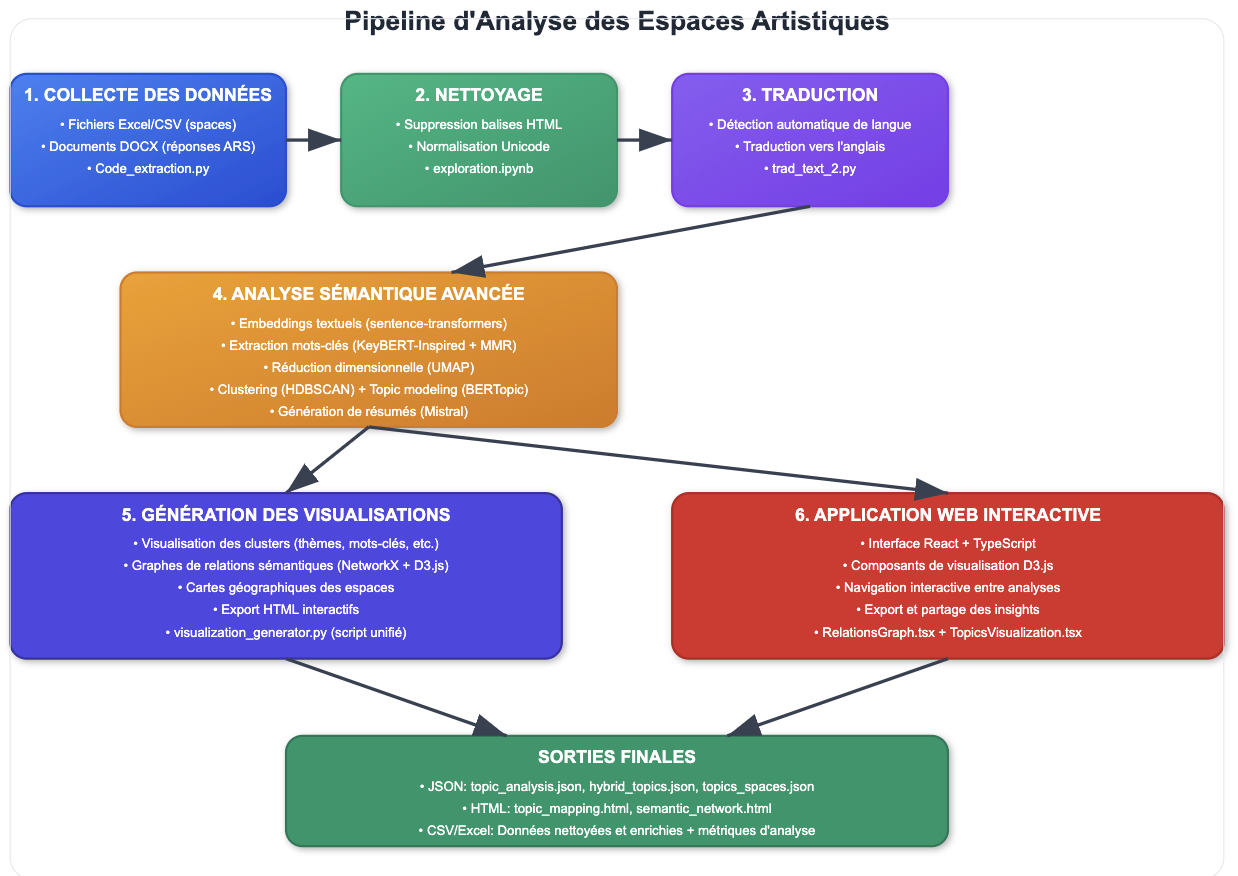
\includegraphics[width=11cm,height=9cm]{Pipeline_diagram.png}
    \caption{Pipeline d'analyse des espaces}
    \label{fig:enquete}
\end{figure}

\hypertarget{analyse-exploratoire-des-donnuxe9es}{%
\chapter{Analyse Exploratoire des Données}\label{analyse-exploratoire-des-donnuxe9es}}

\hypertarget{Contextualisation}{%
\section{Contextualisation}\label{Contextualisation}}

La majorité des visualisations, observations et analyses de données ont été réalisées au cours du premier semestre. Parmi celles-ci figuraient notamment des cartes représentant différents espaces à travers le monde à partir de leurs coordonnées géographiques, ainsi que des boxplots illustrant la durée de vie des espaces.

Au second semestre, nous avons abordé une nouvelle phase centrée sur la modélisation. Celle-ci s’est traduite principalement par la production de nuages de mots, de métriques quantitatives, et de topics accompagnés des mots-clés qui leur sont associés.

Bien que cette approche soit plus abstraite, nous avons néanmoins perçu une réelle utilité dans l’usage des nuages de mots : ils nous ont permis d’identifier rapidement les termes les plus récurrents et de mieux comprendre les éléments saillants présents dans les textes analysés.

\hypertarget{Visualisations des mots des textes}{%
\section{Visualisations des mots des textes}\label{Visualisations des mots des textes}}
Notre exploration des données textuelles s'est déroulée en deux temps, révélant l'importance cruciale du prétraitement dans l'analyse sémantique. Lors de notre première tentative au semestre initial, après les phases conventionnelles de transformation et nettoyage des données, nous avons implémenté la bibliothèque NLTK pour générer des nuages de mots.

Les résultats de cette première approche se sont avérés mitigés. En effet, les visualisations obtenues présentaient plusieurs limitations significatives. D'une part, elles étaient dominées par des termes génériques tels que "art", "artiste" ou "exposition" – vocables certes pertinents dans notre contexte d'étude, mais trop généraux pour faire émerger des thématiques spécifiques et exploitables. D'autre part, ces nuages comportaient également des éléments parasites dénués de signification sémantique comme "X000d" ou "zona", vestiges évidents d'un nettoyage textuel insuffisant.

\begin{figure}[H]
    \centering
    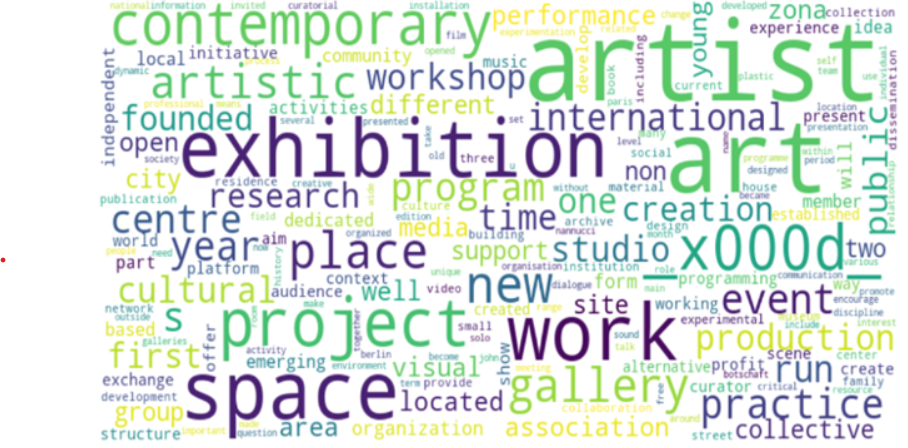
\includegraphics[width=13cm,height=5cm]{ancien_nuage_mots.png}
    \caption{Nuage de mots précédents}
    \label{fig:enquete}
\end{figure}

Face à ces constats, nous avons entrepris de repenser entièrement notre pipeline de traitement textuel au second semestre. Cette refonte a impliqué l'élaboration d'une méthodologie plus sophistiquée, intégrant des techniques d'analyse sémantique avancée. Notre nouvelle approche a notamment inclus une détection plus fine des entités nommées, l'élimination ciblée des termes vides de sens, et l'application de méthodes de lemmatisation contextuelle.

Cette évolution méthodologique a entraîné une amélioration spectaculaire de la qualité de nos visualisations. Le nouveau nuage de mots s'est révélé nettement plus pertinent, faisant émerger des clusters thématiques clairement identifiables. Les termes parasites ont disparu, tandis que la distribution des mots reflète désormais plus fidèlement les nuances du corpus analysé.

\begin{figure}[H]
    \centering
    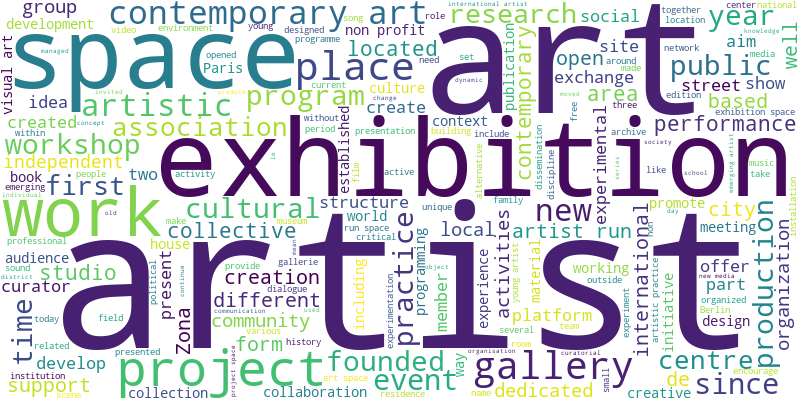
\includegraphics[width=13cm,height=5cm]{word_cloud.png}
    \caption{Nuage de mots des termes les plus fréquents dans les textes des espaces culturels.}
    \label{fig:enquete}
\end{figure}

Cette progression illustre parfaitement l'influence déterminante des méthodes de prétraitement sur la qualité des analyses textuelles. L'extraction de connaissances pertinentes à partir de données non structurées requiert manifestement une attention particulière aux étapes préliminaires, souvent sous-estimées, de la chaîne de traitement. Notre expérience démontre qu'un investissement dans l'optimisation du nettoyage textuel génère des dividendes significatifs en termes d'interprétabilité et de pertinence des résultats.


\hypertarget{analyse-et-ruxe9sultats}{%
\chapter{Analyse et Résultats}\label{analyse-et-ruxe9sultats}}

Cette section présente les résultats obtenus à partir de l’analyse des données textuelles des espaces culturels, en suivant une approche méthodique qui combine des visualisations statistiques, textuelles, thématiques, et sémantiques. Les résultats sont organisés en sous sections pour refléter les différentes étapes de l’analyse, allant des statistiques globales à l’exploration des relations sémantiques entre les espaces. Chaque sous-section inclut des visualisations interactives ou statiques générées à partir des données, accompagnées d’une interprétation détaillée.

\hypertarget{STATISTIQUES GÉNÉRALES ET PARTICIPATION À L'ENQUÊTE}{%
\section{STATISTIQUES GÉNÉRALES ET PARTICIPATION À L'ENQUÊTE }\label{STATISTIQUES GÉNÉRALES ET PARTICIPATION À L'ENQUÊTE }}

\bigskip

\subsection{Statistiques globales des réponses }

\bigskip

Le diagramme circulaire 1-1 montre la proportion d’espaces ayant répondu à au moins une 
question par rapport à ceux sans réponse. On note que seulement 3.8\% des responsables des 
espaces ont répondus à questionnaires. Les réponses issues du questionnaire nous ont permis 
d’enrichir notre base de données textuelle des espaces culturelles. Notre étude se porte sur des 
descriptions d'activités, présentations et historiques des espaces, collectées indépendamment 
des réponses aux questions spécifiques de l'enquête. Ainsi, l'analyse sémantique ne souffre 
pas de ce biais de non-réponse, car elle s'appuie sur des données descriptives préexistantes 
plutôt que sur les réponses directes aux questions.
Par exemple, on peut utiliser un modèle de régression linéaire

\begin{figure}[H]
    \centering
    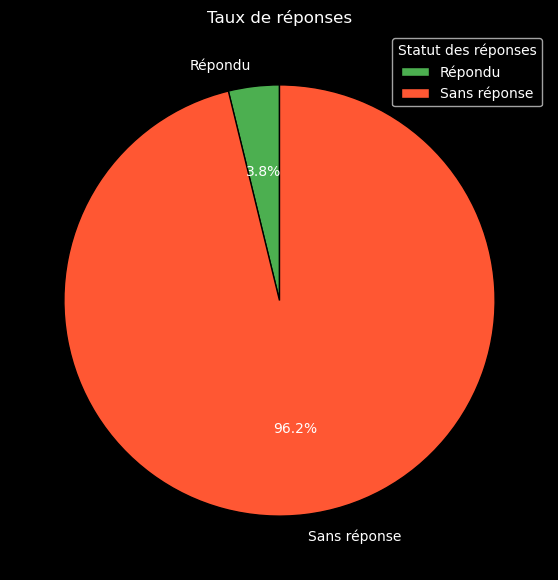
\includegraphics[width=8cm,height=7cm]{Enquete.png}
    \caption{Taux de réponses aux questions posées }
    \label{fig:enquete}
\end{figure}



\bigskip

\subsection{Analyse textuelle globale : Nuage de mots }

\bigskip

Le nuage de mots révèle une hiérarchie claire des concepts centraux dans l'univers des 
espaces artistiques contemporains. Les termes les plus prominents, tels que exhibition, space, 
art, artist, et project, dominent visuellement avec des tailles de police importantes, indiquant 
leur fréquence élevée dans les textes. Ces mots suggèrent que les espaces culturels se 
concentrent principalement sur des activités liées aux expositions, à l’art contemporain, et aux 
projets artistiques, souvent portés par des artistes individuels ou des collectifs. D’autres 
termes comme contemporary, gallery, work, et workshop renforcent cette orientation vers 
des environnements créatifs dynamiques, incluant des ateliers et des galeries. La présence de 
mots comme international, community, et collaboration indique une dimension globale et 
collaborative dans les activités des espaces, tandis que design et production soulignent des 
aspects liés à la création et à la mise en œuvre artistique.



\begin{figure}[H]
    \centering
    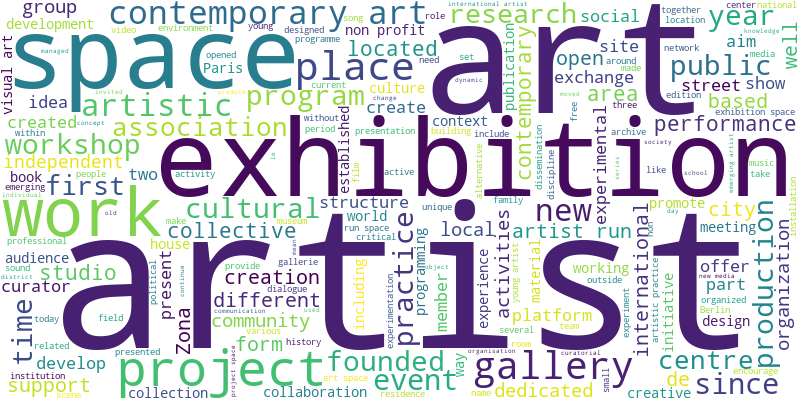
\includegraphics[width=13cm,height=5cm]{word_cloud.png}
    \caption{Nuage de mots des termes les plus fréquents dans les textes des espaces culturels.}
    \label{fig:enquete}
\end{figure}

\section{ANALYSE THÉMATIQUE PAR TOPICS MODELING}

Cette section présente les résultats de l’identification des thématiques des espaces culturels à 
l’aide de BERTopic, ainsi que leur évaluation quantitative. Les thématiques ont été extraites à 
partir des textes prétraités, et leur qualité a été analysée à travers des métriques spécifiques. 

\subsection{Mapping des topics }

Le diagramme 2.1 sunburst interactif des topics, offre une perspective visuelle et hiérarchique 
sur la qualité et la distribution des thématiques identifiées par BERTopic, renforçant 
l’évaluation de leur pertinence et de leur couverture.  
De l’analyse de ce diagramme il ressort que, le topic 0 dominant (environ 30 \% des 
documents), suggérant une thématique générale transversale. Les topics secondaires (1 à 67) 
forment des segments plus petits, indiquant des sous-thèmes spécifiques. Les mots-clés et 
espaces associés (accessibles au survol) confirment le rôle central de Topic 0, potentiellement 
lié à "art" ou "projets". La diversité des couleurs reflète une répartition équilibrée.

\begin{figure}[H]
    \centering
    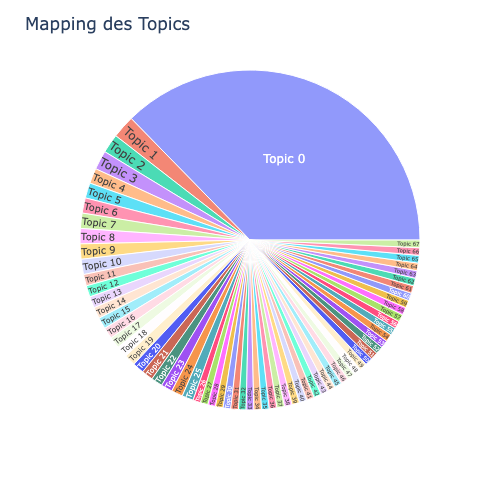
\includegraphics[width=6cm,height=5cm]{MappingTopics.png}
    \caption{Sunburst interactif des topics montrant la répartition et les associations avec les espaces culturels}
    \label{fig:enquete}
\end{figure}

\subsection{Distributions des topics par document }

Le diagramme 2.2 en barres interactif, révèle une distribution déséquilibrée, avec Topic 0 
dominant (37\% des documents), suggérant une thématique très générale ( art ou exposition). 
Les autres topics (1 à 67) affichent des pourcentages négligeables (<1 \%), suggérant des 
thématiques spécifiques mais peu représentées dans les données. indiquant une faible 
granularité due aux paramètres HDBSCAN (min\_cluster\_size=2). 
Le topic 0, dominant avec 37,3\% des documents, reflète une thématique centrale, mais 
suggère une homogénéité potentiellement générique. Les topics secondaires (1 à 25), 
variant de 2 \% à 0,7 \%, montrent une diversité thématique, certains étant bien représentés 
(topic 1, d’autres marginaux (topic 26, 2 documents). Le survol des segments révèle des 
associations spécifiques entre les topics et les pourcentages de documents.


\begin{figure}[H]
    \centering
    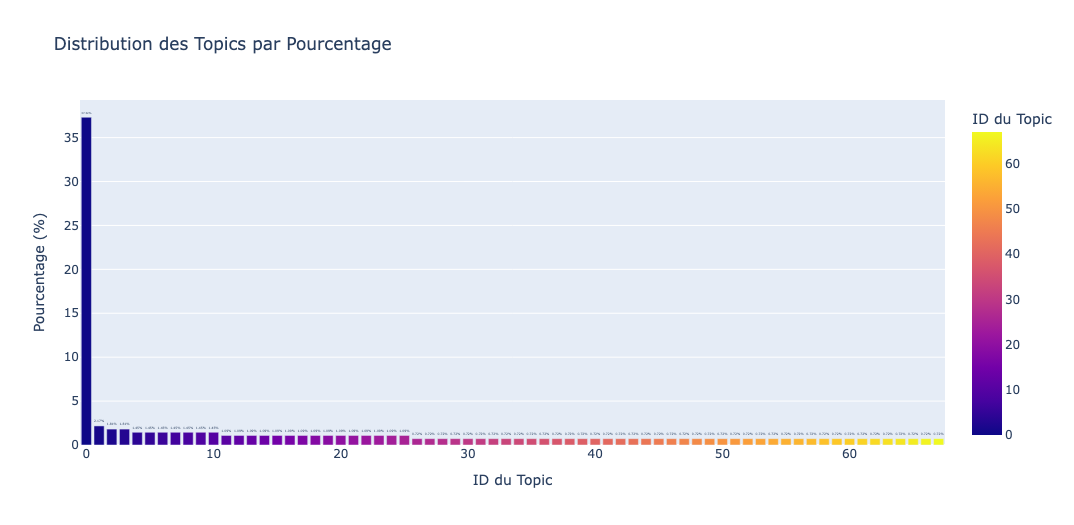
\includegraphics[width=14cm,height=7cm]{DistributionParDoc.png}
    \caption{Distribution des topics par pourcentage de documents dans les textes des espaces culturels. }
    \label{fig:enquete}
\end{figure}

\section{Analyse qualitative des topics et Évaluations des topics }

Cette section évalue la qualité des topics identifiés par BERTopic à travers une analyse 
qualitative et quantitative, en examinant leur cohérence sémantique et leur diversité 
thématique. Des métriques spécifiques ont été calculées pour mesurer la performance du 
modèle, notamment la proportion de documents non assignés (topic -1), la diversité des 
topics, et leur couverture. Ces résultats permettent d’apprécier la robustesse du clustering 
thématique et de valider l’adéquation des topics pour une analyse fine des espaces culturels.

\subsection{Cohérence sémantique et diversité thématique }

L’analyse qualitative des topics s’est concentrée sur deux aspects clés : la cohérence 
sémantique et la diversité thématique. 

\begin{itemize}
    \item Cohérence sémantique :
    
    La cohérence sémantique a été évaluée en examinant les mots-clés générés pour chaque topic (via KeyBERTInspired et MMR) et les résumés produits par Mistral Small 3.1, disponibles dans hybrid\_topics.json. Les topics montrent une cohérence sémantique satisfaisante, car les mots-clés associés à chaque topic (par exemple, "art", "exhibition", "project" pour Topic 0, comme observé dans le nuage de mots) forment des ensembles thématiques cohérents et  interprétables. Les résumés générés confirment cette cohérence en synthétisant les thématiques principales de manière concise et pertinente.

    \bigskip
    
    \item Diversité thématique :

     La diversité des topics a été mesurée à l’aide de la métrique de diversité, qui évalue la redondance des mots-clés entre les topics. Une valeur élevée (proche de 1) indique une faible redondance et donc une grande diversité thématique. Comme indiqué dans le tableau ci-dessous, la diversité des topics atteint 0,913, une valeur très proche de l’idéal (1). Cela signifie que les topics sont distincts les uns des autres, avec un minimum de chevauchement sémantique, ce qui reflète la capacité du modèle à capturer une large variété de thématiques au sein des données des espaces culturels.
\end{itemize}

\subsection{ Évaluation quantitative des topics}

Les métriques quantitatives suivantes ont été calculées pour évaluer la performance du modèle BERTopic. Ces métriques incluent le pourcentage de documents non assignés (topic 1), la diversité des topics, et la couverture des topics. Les résultats sont résumés dans le tableau ci-dessous et ont été sauvegardés dans le fichier quality\_metrics.json pour une utilisation ultérieure dans React. 


\begin{table}[h]
    \centering
    \caption{Métriques de performance des topics}
    \begin{tabular}{|p{4cm}|p{2.5cm}|p{7cm}|}
        \hline
        \textbf{Métrique} & \textbf{Valeur} & \textbf{Interprétation} \\
        \hline
        Pourcentage de documents dans le topic -1 & 10,10\% & 10,1\% des documents ne sont pas assignés à un topic, ce qui est acceptable mais pourrait être amélioré. \\
        \hline
        Diversité des topics & 0,913 & Diversité des topics 0,913 vaut proche de 1, indiquant une grande diversité thématique avec une redondance minimale des mots-clés. \\
        \hline
        Couverture des topics & 0,101 & 89,9\% des textes sont bien couverts par les 68 topics, une performance adaptée à une analyse fine. \\
        \hline
    \end{tabular}
    \label{tab:topic_metrics}
\end{table}

\bigskip
Conclusion : 

L’analyse qualitative et quantitative des topics montre que le modèle BERTopic a réussi à produire des topics cohérents et diversifiés, avec une couverture acceptable des données. La cohérence sémantique est satisfaisante, comme en témoignent les mots-clés et résumés, tandis que la diversité thématique élevée (0,913) garantit une bonne différenciation des topics. Cependant, le pourcentage de documents non assignés (10,1 \%) suggère qu’un ajustement des paramètres (par exemple, min\_cluster\_size dans HDBSCAN) ou une amélioration du prétraitement des textes pourrait optimiser davantage les résultats. Ces métriques confirment la pertinence du modèle pour une analyse thématique des espaces culturels, tout en identifiant des axes d’amélioration pour de futures itérations.


\section{Analyse des relation sémantiques entre topics. }

Les relations entre les topics ont été explorées à travers plusieurs visualisations 
complémentaires, offrant une vue multidimensionnelle de leur organisation sémantique. Ces 
analyses, réalisées avec BERTopic et Plotly, permettent de comprendre les similarités, les 
hiérarchies, et les distributions des thématiques, enrichissant l’interprétation des résultats 
thématiques.

\subsection{Carte des distances entre topics }


La carte des distances (figure 4.1), montrant une représentation interactive en 2D projette les 
centroïdes des topics, où chaque point (ou cercle) représente un topic, la taille du cercle est 
proportionnelle au nombre de documents associés, et la distance entre les points reflète la 
dissimilarité sémantique basée sur la distance cosinus des embeddings. 
L’analyse de la carte des distances révèle une organisation spatiale des topics en plusieurs 
clusters distincts. Un groupe dense de topics se concentre dans la moitié bas à droite du 
graphique, suggérant une forte similarité sémantique entre ces thématiques, probablement 
liées à des concepts communs comme art ou exposition, comme observé dans le nuage de 
mots. La taille variable des cercles indique une disparité dans le nombre de documents, avec 
un topic central plus large (par exemple, Topic 0) dominant ce cluster. À l’opposé, des topics 
isolés comme Topic  46,54 et 65, situés à gauche, apparaissent comme des thématiques plus 
distinctes, potentiellement des outliers ou des sujets spécifiques. Cette distribution reflète une 
diversité thématique, mais la proximité des topics dans le cluster principal suggère un 
chevauchement sémantique qui pourrait être affiné par un ajustement des paramètres UMAP 
ou HDBSCAN. Cette visualisation confirme la présence de relations sémantiques.  


\begin{figure}[H]
    \centering
    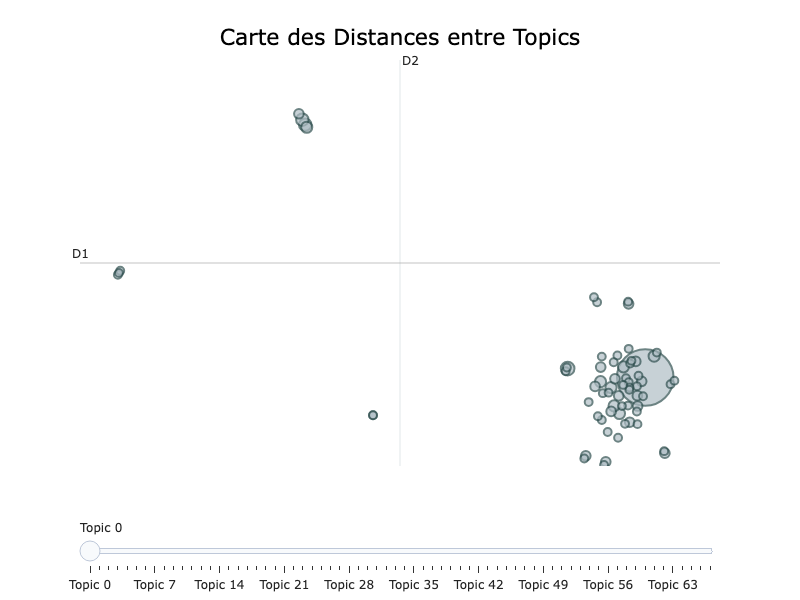
\includegraphics[width=15cm,height=8cm]{CarteDistance.png}
    \caption{Carte des distances entre topics}
    \label{fig:enquete}
\end{figure}

\subsection{Hiérarchie des topics}

La visualisation hiérarchie des topics, montre les relations parent-enfant entre les topics, 
basées sur leur similarité sémantique, avec des nœuds interconnectés et des mots-clés associés 
pour chaque topic.( Distance faible (<5\%, donc forte similarité ; >1, dissimilaire)  
Le dendrogramme met en évidence des regroupements thématiques clairs basés sur la 
similarité sémantique. Les clusters de même couleur sont considérés comme appartenant à 
une même thématique générale, même si certains topics ne sont pas directement très 
similaires ; leur proximité résulte de leur appartenance à un groupe global défini par des 
relations hiérarchiques. Par exemple, les topics 0 et 3 fusionnent à une distance d’environ 0,5, 
révélant une forte similarité sémantique. Ces deux topics semblent partager un noyau 
thématique centré sur la pratique artistique concrète et l’organisation de projets culturels. En 
revanche, des topics comme 25 et 59 ne se rejoignent qu’à une distance supérieure à 0,9, 
indiquant une dissimilarité marquée malgré une éventuelle proximité lexicale. Cette capacité 
du modèle à capturer des nuances sémantiques profondes au-delà des simples mots partagés 
confirme la robustesse de l’approche hiérarchique, offrant une vue détaillée des relations 
thématiques au sein des données.


\begin{figure}[H]
    \centering
    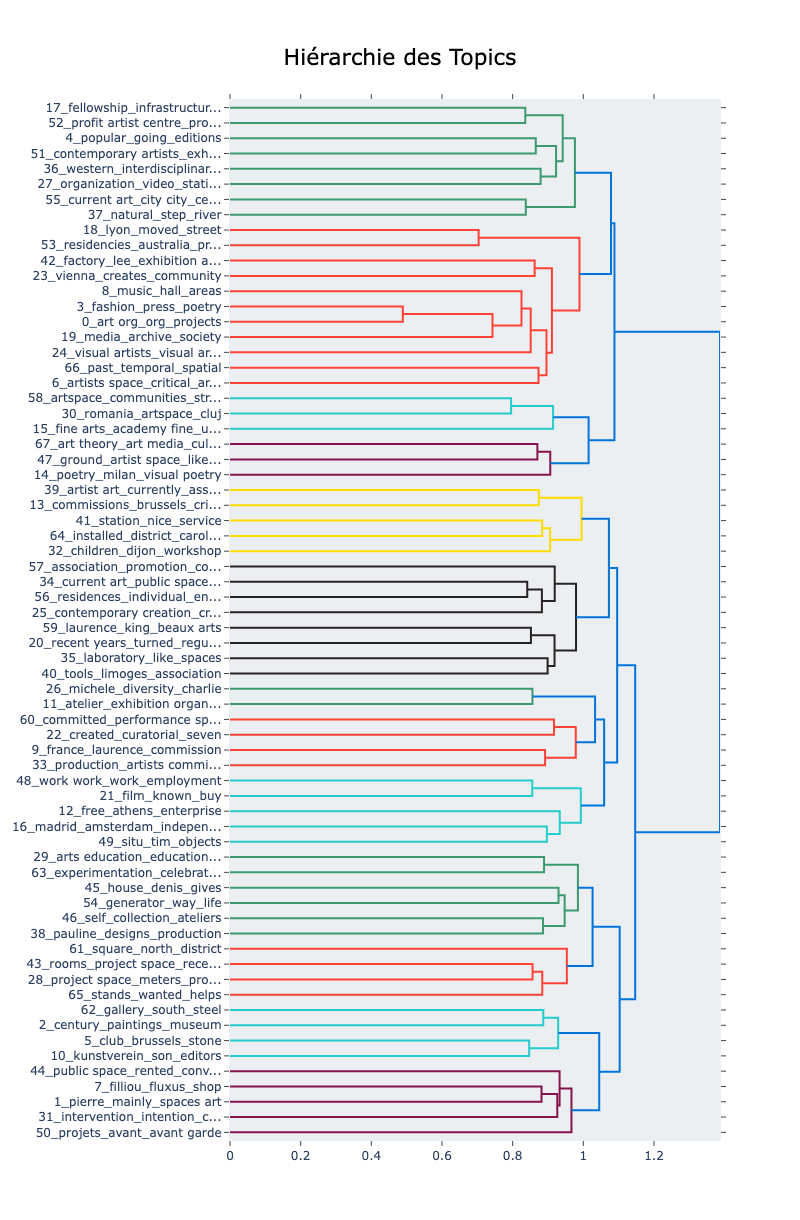
\includegraphics[width=14cm,height=8cm]{Hierachy.png}
    \caption{Hiérarchie des topics }
    \label{fig:enquete}
\end{figure}

\subsection{Distribution des mots-clés par topic}


Les graphiques en barres (figure 4.3), montre les mots-clés les plus fréquents par topic, avec 
des fréquences normalisées sur l’axe y 
L’analyse des distributions des mots-clés révèle des profils thématiques distincts pour chaque 
topic. Par exemple, Topic 0 met en avant des termes comme art, org, et projects, indiquant 
une thématique centrée sur l’organisation artistique, tandis que Topic 1 privilégie people, 
museum, et modern, suggérant un focus sur les institutions culturelles. Topic 6, avec art 
space et artwork, se concentre sur les espaces d’exposition, et Topic 15, avec fine arts et 
academy, sur l’éducation artistique. La variation des hauteurs des barres montre une 
dominance de certains mots-clés par topic, reflétant une cohérence interne, mais aussi une 
certaine redondance (par exemple, art apparaît dans plusieurs topics). Cette visualisation 
valide la diversité thématique observée dans la diversité des topics (0,913) et souligne 
l’importance d’examiner les mots-clés pour affiner les interprétations sémantiques.


\begin{figure}[H]
    \centering
    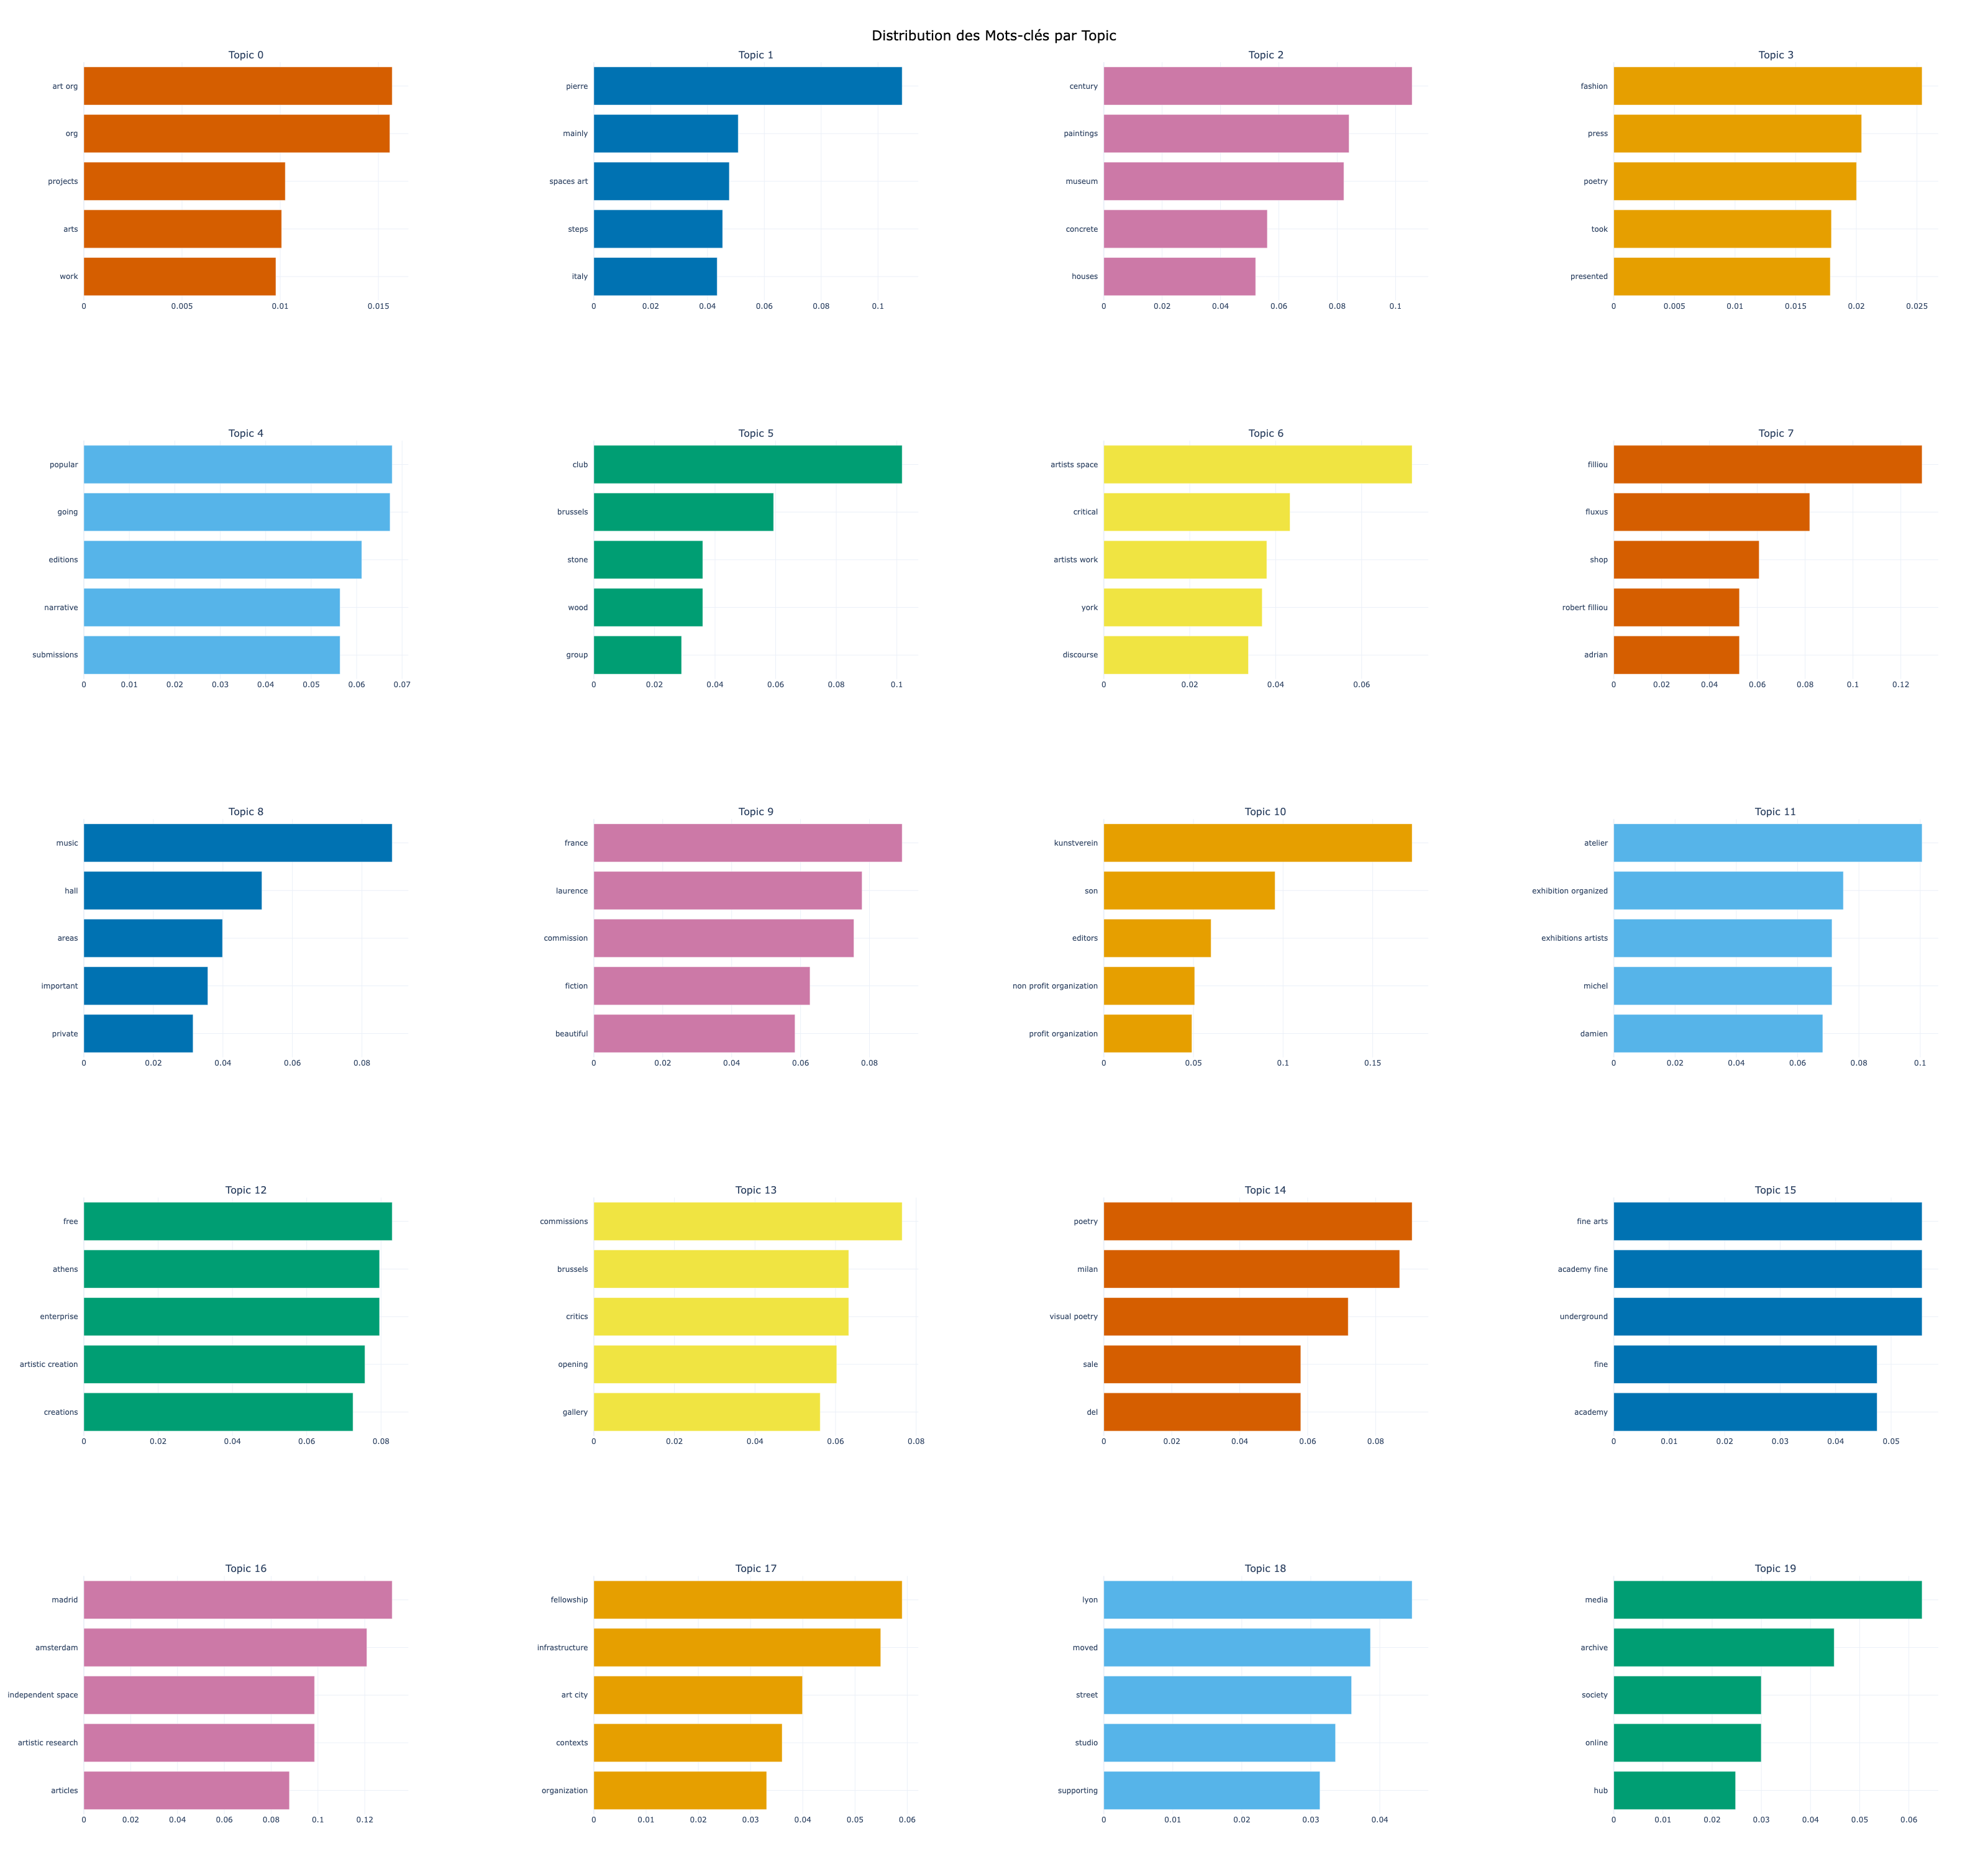
\includegraphics[width=15cm,height=8cm]{distributions.png}
    \caption{Distribution des mots-clés par topic }
    \label{fig:enquete}
\end{figure}

\subsection{ Heatmap de similarité entre topics}

La matrice (figure 4.4) utilise la similarité cosinus entre les centroïdes des topics, avec une 
échelle de couleur allant de 0,4 (faible similarité) à 0,9 (forte similarité). 
La heatmap illustre les relations sémantiques entre les topics à travers leurs similarités 
cosinus. Comme attendu, la diagonale affiche une similarité de 1,0 (en bleu foncé), car chaque 
topic est parfaitement similaire à lui-même. Hors diagonale, des blocs de forte similarité (en 
bleu, autour de 0,8-0,9) émergent, notamment entre Topic 0 ( art org, projects) et Topic 4 
(popular going, editions), suggérant un chevauchement thématique lié à l’organisation 
artistique et aux projets culturels. De même, Topic 15 (fine arts, academy) et Topic 12 
(commission, artists) montrent une corrélation élevée, indiquant des liens potentiels dans les 
domaines éducatif et professionnel de l’art. À l’inverse, de nombreuses paires de topics 
affichent une faible similarité (en vert clair, autour de 0,4-0,5), confirmant une diversité 
thématique globale, cohérente avec la métrique de diversité (0,913). Ces résultats corroborent 
les clusters observés dans la carte des distances (section 7.6.1), mais soulignent également la 
nécessité d’affiner les paramètres du modèle pour réduire les redondances entre topics 
fortement corrélés.


\begin{figure}[H]
    \centering
    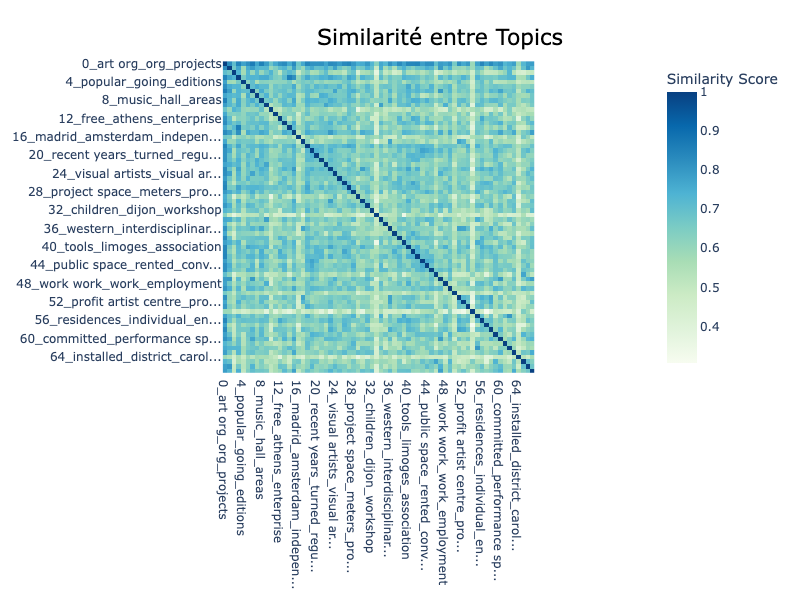
\includegraphics[width=16cm,height=9cm]{Heatmap.png}
    \caption{Heatmap de similarité entre topics}
    \label{fig:enquete}
\end{figure}

\bigskip

Conclusion :  


Les visualisations complémentaires montrent une organisation sémantique riche et variée des 
topics. La carte des distances identifie des clusters et des outliers, la hiérarchie révèle des 
relations parent-enfant cohérentes, les distributions des mots-clés confirment la spécificité 
thématique, et la heatmap met en évidence des similarités significatives. Ces analyses 
suggèrent une structure thématique complexe, avec des thématiques dominantes (comme l’art 
et les projets) et des sous-thèmes spécifiques. 

\section{Relations sémantiques entre espaces}

Cette section explore les relations sémantiques entre les espaces culturels à travers la 
construction d’un graphe de similarité thématique, permettant d’identifier les groupes 
d’espaces partageant des thématiques communes. Deux visualisations ont été générées : un 
graphe statique pour une vue d’ensemble et un graphe interactif pour une exploration 
détaillée. Ces analyses s’appuient sur les embeddings moyens des espaces, et sur la similarité 
cosinus pour établir les connexions. 
Le graph sémantique non orienté (figure 5), représente les relations entre les espaces culturels, 
où les nœuds correspondent aux espaces, les arêtes aux similarités sémantiques fortes (basées 
sur la similarité cosinus des embeddings moyens, avec un seuil calculé dynamiquement à 
0,492), et les couleurs indiquent les topics associés.  
L’analyse du graphe sémantique révèle une structure relationnelle riche entre les espaces 
culturels, mettant en évidence des clusters thématiques distincts.


\subsection{Graphe statique }

Le graphe statique affiche un réseau dense avec de multiples connexions, où les nœuds sont 
colorés selon les topics (de 0 à 67, hors -1) à l’aide d’une palette rainbow. Les arêtes, 
représentant des similarités cosinus supérieures au seuil dynamique de 0,492, connectent les 
espaces partageant des thématiques proches. Un cluster central dense est observable, 
probablement dominé par des thématiques générales comme art ou exposition (liées à Topic 
0), tandis que des sous-groupes périphériques, colorés différemment, suggèrent des 
thématiques plus spécifiques. La densité élevée des connexions dans le centre reflète une forte 
cohésion thématique au sein de ce groupe, tandis que les arêtes plus rares vers les périphéries 
indiquent une diversification des sujets.


\begin{figure}[H]
    \centering
    \includegraphics[width=15cm,height=10cm]{semantic_network_spaces.png}
    \caption{Graphe sémantique statique des relations entre espaces culturels. }
    \label{fig:enquete}
\end{figure}

\subsection{Graphe interactif }

La version interactive dans React permet une exploration détaillée du réseau sémantique, 
composé de 220 nœuds (espaces culturels) et 3312 arêtes (connexions), avec une densité de 
0,143 pour un seuil de similarité cosinus de 0,492. Cette densité, correspondant à 14,3 \% des 
connexions possibles, reflète une connectivité modérée mais significative, adaptée à un seuil 
relativement strict. Il est important de noter que ce seuil peut être ajusté : un seuil plus bas 
augmenterait le nombre de connexions et la densité, révélant davantage de relations 
sémantiques, tandis qu’un seuil plus élevé réduirait les arêtes, isolant davantage les clusters 
thématiques. Les nœuds sont étiquetés avec les noms des espaces et colorés selon les topics 
associés (par exemple, bleu pour Topic 0, vert pour Topic 15). Le cluster central, dominé par 
des thématiques artistiques générales (bleu), regroupe des espaces fortement interconnectés, 
tandis que des sous-groupes ou nœuds isolés (vert ou rouge) reflètent des thématiques 
spécifiques comme l’éducation artistique ou les ateliers. L’interactivité permet de repérer des 
espaces clés : par exemple, Collective et Corridor Project Space, chacun avec 25 
connexions, se distinguent comme des hubs thématiques, jouant un rôle central dans leurs 
réseaux respectifs.

\begin{figure}[H]
    \centering
    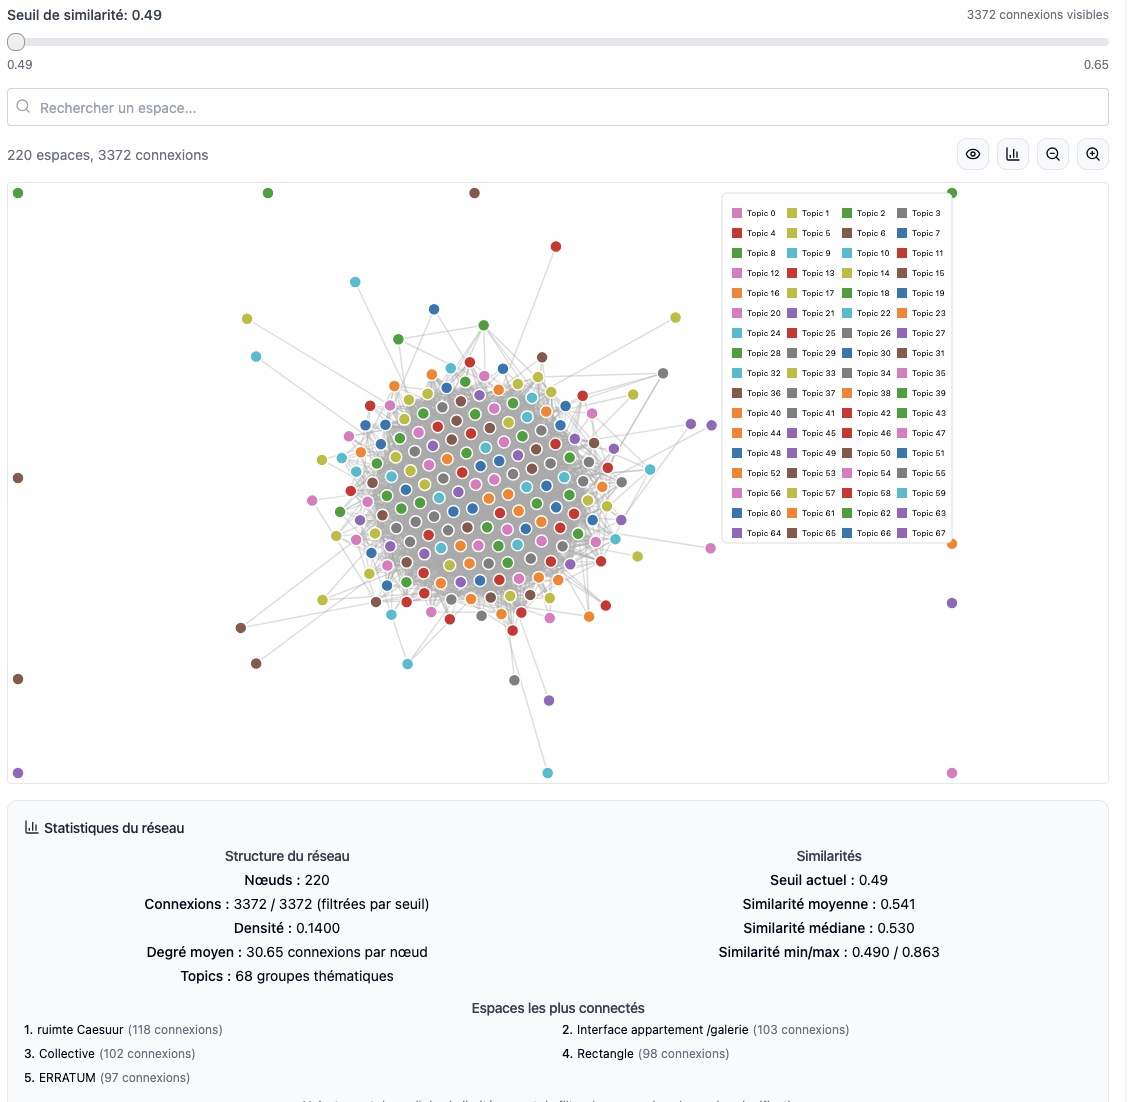
\includegraphics[width=15cm,height=8cm]{semantic_network_spaces2.png}
    \caption{Graphe sémantique interactif des relations entre espaces culturels. }
    \label{fig:enquete}
\end{figure}

\hypertarget{discussion}{%
\chapter{Discussion}\label{discussion}}

Suite aux observations, statistiques et modèles nous avons obtenu de nombreux résultats. Nous avons donc choisi de prendre le modèle BERTopic (en s'appuyant sur le modèle de représentation KeyBERTInspired+MMR) qui nous génère un grand nombre de topics, eux mêmes interprétés par une intégration Mistral. Ce grand nombre de topics (69) nous est très favorable, en effet le fait d'avoir beaucoup de topics (69 sur 330 espaces) nous permet d'avoir nos espaces représentés selon des caractéristiques propre à eux mêmes mais aussi en relation aux autres. C'est exactement ce que l'on voulait à la base, pouvoir faire ressortir l'essence d'un espace d'art pour pouvoir le rapprocher a un thème spécial qui coïncide avec d'autres espaces et non pas trouver des thèmes généraux qui englobent beaucoup d'espaces et qui ne sont pas très pertinents pour les espaces qu'il englobe. De plus notre pipeline de traitement incluant le traitement des données, la traduction et le modèle permettra à nos commanditaires de pouvoir ajouter des espaces et des descritpions pour relancer l'analyse et générer de nouveaux topics.

\bigskip

La taille limitée de notre base de données textuelles, comprenant seulement 330 espaces culturels, restreint la portée de l’analyse. Une augmentation du nombre d’espaces aurait permis d’enrichir l’étude en capturant une plus grande diversité thématique. Par ailleurs, le faible taux de réponse au questionnaire de nombreux espaces a réduit la quantité de données disponibles pour ces 330 entités, limitant ainsi la profondeur des insights potentiellement tirés de cette population.

Malgré les résultats prometteurs, quelques limites méritent d’être adressées. L’ajustement manuel des paramètres (par exemple, min\_cluster\_size dans HDBSCAN ou le seuil de similarité de 0,492 dans le graphe) a influencé les résultats, introduisant une subjectivité dans l’analyse. De plus, la densité modérée du réseau (0,143) et les chevauchements thématiques (observés dans la heatmap) suggèrent que le modèle pourrait sur-clusteriser ou sous-séparer certains topics. Enfin, l’absence d’étiquettes manuelles pour valider les topics limite la confiance dans leur interprétation sémantique, ce qui pourrait être amélioré par une évaluation humaine.

\hypertarget{conclusion-et-perspectives}{%
\chapter{Conclusion et perspectives}\label{conclusion-et-perspectives}}

Ce projet TER nous a permis d'explorer en profondeur un cas concret d’analyse textuelle à grande échelle, en mettant en œuvre des outils avancés de la data science, tout en nous confrontant aux réalités de la gestion d’un projet collaboratif.

Sur le plan technique, nous avons acquis des compétences dans le traitement de données textuelles multilingues, en combinant plusieurs étapes : nettoyage linguistique, normalisation, traduction, vectorisation, clustering sémantique, et visualisation. L’usage de BERTopic nous a amenés à comprendre la complexité du topic modeling moderne, notamment l’importance du choix des embeddings, des paramètres de réduction de dimension, et des algorithmes de clustering. Nous avons appris à évaluer la qualité des modèles à travers des métriques telles que la diversité thématique ou la couverture des documents, mais aussi à interpréter les résultats de façon critique, en lien avec notre sujet d’étude.

Ce projet a également été l’occasion d’utiliser des outils et bibliothèques reconnus du domaine tels que SpaCy, sentence-transformers, HDBSCAN, UMAP, Plotly et NetworkX, et de réfléchir à leur articulation dans un pipeline reproductible. Nous avons ainsi développé une vraie démarche analytique, alliant exploration, modélisation et mise en récit des résultats.

Sur le plan de la gestion de projet, l’organisation agile que nous avons adoptée, avec ses itérations courtes et ses réunions hebdomadaires, nous a appris à planifier, prioriser, et surtout à réagir face aux imprévus. Le suivi des tâches, l’utilisation de GitHub pour la traçabilité, et l’engagement de chacun dans la dynamique collective ont été essentiels à notre réussite.
Enfin, nous avons particulièrement apprécié l’évolution de notre communication, tant en interne qu’avec notre tuteur. L’implication de M. Collin, en particulier dans les dernières semaines, a grandement contribué à clarifier certaines étapes techniques clés et à élever la qualité de notre travail. Nous lui exprimons notre gratitude pour le temps, l’expertise et la disponibilité qu’il nous a consacrés.

En somme, ce projet a constitué une expérience formatrice complète, tant sur le plan technique que humain, et nous a préparés concrètement à des missions futures en science des données, où rigueur méthodologique, capacité d’analyse et collaboration seront tout aussi essentielles.

Tout de même nous avons eu de nombreux problèmes et contre temps durant ce projet nous ayant empêché de réaliser tout ce que nous voulions. En effet, nous avions pour objectif de proposer des annotations précises mais par faute de temps nous n'avons pas pu pousser cela jusqu'au bout.
Une extension prometteuse serait l’utilisation de l’algorithme de Louvain pour détecter des communautés au sein du graphe sémantique. Cet algorithme, basé sur une optimisation de la modularité, fonctionne en deux étapes principales : (1) il attribue initialement chaque nœud (espace) à une communauté distincte, puis (2) itère sur les nœuds pour les regrouper avec leurs voisins si cela augmente la modularité (une mesure de la qualité des partitions). Ce processus se répète à différentes échelles jusqu’à convergence, identifiant des sous-groupes denses de manière hiérarchique. Appliqué au graphe des espaces, Louvain pourrait révéler des communautés thématiques plus fines que les clusters actuels, par exemple des groupes d’espaces spécialisés dans l’éducation artistique ou les ateliers, au-delà des topics préalablement définis par BERTopic. Cela pourrait aider à mieux comprendre les dynamiques locales entre espaces et à proposer des recommandations ciblées pour des collaborations ou des événements culturels.

\bigskip

\hypertarget{bibliographie}{%
\chapter*{Bibliographie}\label{bibliographie}}
\addcontentsline{toc}{chapter}{Bibliographie}

\hypertarget{refs}{}
\begin{CSLReferences}{0}{0}

\leavevmode\hypertarget{ref-ARS}{}%
\textbullet\ Equipe artist-run spaces, 2025. \emph{Projet de TER Artist-run spaces.} 

Disponible en ligne à l'adresse : \url{https://github.com/vitamineeo/Projet-TER-artiste-run-spaces}

\vspace{0.8em}

\leavevmode\hypertarget{ref-pradeep}{}%
\textbullet\ Pradeep. 01 May, 2025. \emph{Keyword Extraction Methods from Documents in NLP.} 

Disponible en ligne à l'adresse : \url{https://www.analyticsvidhya.com/blog/2022/03/keyword-extraction-methods-from-documents-in-nlp/}

\vspace{0.8em}

\leavevmode\hypertarget{ref-python}{}%
\textbullet\ Python Software Foundation. ©2001--2025. \emph{unittest — Unit testing framework.}  

Disponible en ligne à l'adresse : \url{https://docs.python.org/3/library/unittest.html}

\vspace{0.8em}

\leavevmode\hypertarget{ref-bertopic}{}%
\textbullet\ Grootendorst, Maarten. ©2024. \emph{Guided Topic Modeling.}  

Disponible en ligne à l'adresse : \url{https://maartengr.github.io/BERTopic/getting_started/guided/guided.html}

\vspace{0.8em}

\leavevmode\hypertarget{ref-jupytext}{}%
\textbullet\ Jupytext Team. ©2018--2023. \emph{Notebooks as code.}  

Disponible en ligne à l'adresse : \url{https://jupytext.readthedocs.io/en/latest/formats-scripts.html}

\end{CSLReferences}


\end{document}

